% Options for packages loaded elsewhere
\PassOptionsToPackage{unicode}{hyperref}
\PassOptionsToPackage{hyphens}{url}
\PassOptionsToPackage{dvipsnames,svgnames,x11names}{xcolor}
%
\documentclass[
  11,
  a4paper,
]{article}

\usepackage{amsmath,amssymb}
\usepackage{setspace}
\usepackage{iftex}
\ifPDFTeX
  \usepackage[T1]{fontenc}
  \usepackage[utf8]{inputenc}
  \usepackage{textcomp} % provide euro and other symbols
\else % if luatex or xetex
  \usepackage{unicode-math}
  \defaultfontfeatures{Scale=MatchLowercase}
  \defaultfontfeatures[\rmfamily]{Ligatures=TeX,Scale=1}
\fi
\usepackage{lmodern}
\ifPDFTeX\else  
    % xetex/luatex font selection
  \setmainfont[Numbers=Lowercase,Numbers=Proportional]{Times New Roman}
\fi
% Use upquote if available, for straight quotes in verbatim environments
\IfFileExists{upquote.sty}{\usepackage{upquote}}{}
\IfFileExists{microtype.sty}{% use microtype if available
  \usepackage[]{microtype}
  \UseMicrotypeSet[protrusion]{basicmath} % disable protrusion for tt fonts
}{}
\makeatletter
\@ifundefined{KOMAClassName}{% if non-KOMA class
  \IfFileExists{parskip.sty}{%
    \usepackage{parskip}
  }{% else
    \setlength{\parindent}{0pt}
    \setlength{\parskip}{6pt plus 2pt minus 1pt}}
}{% if KOMA class
  \KOMAoptions{parskip=half}}
\makeatother
\usepackage{xcolor}
\usepackage[top=15mm,left=22.5mm,right=22.5mm,bottom=15mm]{geometry}
\setlength{\emergencystretch}{3em} % prevent overfull lines
\setcounter{secnumdepth}{-\maxdimen} % remove section numbering
% Make \paragraph and \subparagraph free-standing
\ifx\paragraph\undefined\else
  \let\oldparagraph\paragraph
  \renewcommand{\paragraph}[1]{\oldparagraph{#1}\mbox{}}
\fi
\ifx\subparagraph\undefined\else
  \let\oldsubparagraph\subparagraph
  \renewcommand{\subparagraph}[1]{\oldsubparagraph{#1}\mbox{}}
\fi


\providecommand{\tightlist}{%
  \setlength{\itemsep}{0pt}\setlength{\parskip}{0pt}}\usepackage{longtable,booktabs,array}
\usepackage{calc} % for calculating minipage widths
% Correct order of tables after \paragraph or \subparagraph
\usepackage{etoolbox}
\makeatletter
\patchcmd\longtable{\par}{\if@noskipsec\mbox{}\fi\par}{}{}
\makeatother
% Allow footnotes in longtable head/foot
\IfFileExists{footnotehyper.sty}{\usepackage{footnotehyper}}{\usepackage{footnote}}
\makesavenoteenv{longtable}
\usepackage{graphicx}
\makeatletter
\def\maxwidth{\ifdim\Gin@nat@width>\linewidth\linewidth\else\Gin@nat@width\fi}
\def\maxheight{\ifdim\Gin@nat@height>\textheight\textheight\else\Gin@nat@height\fi}
\makeatother
% Scale images if necessary, so that they will not overflow the page
% margins by default, and it is still possible to overwrite the defaults
% using explicit options in \includegraphics[width, height, ...]{}
\setkeys{Gin}{width=\maxwidth,height=\maxheight,keepaspectratio}
% Set default figure placement to htbp
\makeatletter
\def\fps@figure{htbp}
\makeatother
\newlength{\cslhangindent}
\setlength{\cslhangindent}{1.5em}
\newlength{\csllabelwidth}
\setlength{\csllabelwidth}{3em}
\newlength{\cslentryspacingunit} % times entry-spacing
\setlength{\cslentryspacingunit}{\parskip}
\newenvironment{CSLReferences}[2] % #1 hanging-ident, #2 entry spacing
 {% don't indent paragraphs
  \setlength{\parindent}{0pt}
  % turn on hanging indent if param 1 is 1
  \ifodd #1
  \let\oldpar\par
  \def\par{\hangindent=\cslhangindent\oldpar}
  \fi
  % set entry spacing
  \setlength{\parskip}{#2\cslentryspacingunit}
 }%
 {}
\usepackage{calc}
\newcommand{\CSLBlock}[1]{#1\hfill\break}
\newcommand{\CSLLeftMargin}[1]{\parbox[t]{\csllabelwidth}{#1}}
\newcommand{\CSLRightInline}[1]{\parbox[t]{\linewidth - \csllabelwidth}{#1}\break}
\newcommand{\CSLIndent}[1]{\hspace{\cslhangindent}#1}

\usepackage{lscape}
\newcommand{\blandscape}{\begin{landscape}}
\newcommand{\elandscape}{\end{landscape}}
\makeatletter
\makeatother
\makeatletter
\makeatother
\makeatletter
\@ifpackageloaded{caption}{}{\usepackage{caption}}
\AtBeginDocument{%
\ifdefined\contentsname
  \renewcommand*\contentsname{Table of contents}
\else
  \newcommand\contentsname{Table of contents}
\fi
\ifdefined\listfigurename
  \renewcommand*\listfigurename{List of Figures}
\else
  \newcommand\listfigurename{List of Figures}
\fi
\ifdefined\listtablename
  \renewcommand*\listtablename{List of Tables}
\else
  \newcommand\listtablename{List of Tables}
\fi
\ifdefined\figurename
  \renewcommand*\figurename{Figure}
\else
  \newcommand\figurename{Figure}
\fi
\ifdefined\tablename
  \renewcommand*\tablename{Table}
\else
  \newcommand\tablename{Table}
\fi
}
\@ifpackageloaded{float}{}{\usepackage{float}}
\floatstyle{ruled}
\@ifundefined{c@chapter}{\newfloat{codelisting}{h}{lop}}{\newfloat{codelisting}{h}{lop}[chapter]}
\floatname{codelisting}{Listing}
\newcommand*\listoflistings{\listof{codelisting}{List of Listings}}
\makeatother
\makeatletter
\@ifpackageloaded{caption}{}{\usepackage{caption}}
\@ifpackageloaded{subcaption}{}{\usepackage{subcaption}}
\makeatother
\makeatletter
\@ifpackageloaded{tcolorbox}{}{\usepackage[skins,breakable]{tcolorbox}}
\makeatother
\makeatletter
\@ifundefined{shadecolor}{\definecolor{shadecolor}{rgb}{.97, .97, .97}}
\makeatother
\makeatletter
\makeatother
\makeatletter
\makeatother
\ifLuaTeX
  \usepackage{selnolig}  % disable illegal ligatures
\fi
\IfFileExists{bookmark.sty}{\usepackage{bookmark}}{\usepackage{hyperref}}
\IfFileExists{xurl.sty}{\usepackage{xurl}}{} % add URL line breaks if available
\urlstyle{same} % disable monospaced font for URLs
\hypersetup{
  pdftitle={The genomic landscape of Acute Respiratory Distress Syndrome: a meta-analysis by information content of genome-wide studies of the host response.},
  colorlinks=true,
  linkcolor={blue},
  filecolor={Maroon},
  citecolor={Blue},
  urlcolor={Blue},
  pdfcreator={LaTeX via pandoc}}

\title{The genomic landscape of Acute Respiratory Distress Syndrome: a
meta-analysis by information content of genome-wide studies of the host
response.}
\author{}
\date{}

\begin{document}
\maketitle
\ifdefined\Shaded\renewenvironment{Shaded}{\begin{tcolorbox}[interior hidden, frame hidden, boxrule=0pt, borderline west={3pt}{0pt}{shadecolor}, breakable, enhanced, sharp corners]}{\end{tcolorbox}}\fi

\setstretch{1.5}
Jonathan E Millar\textsuperscript{1,2}, Sara
Clohisey-Hendry\textsuperscript{1,2}, Megan McMannus\textsuperscript{1},
Marie Zechner\textsuperscript{1}, Bo Wang\textsuperscript{1}, Nick
Parkinson\textsuperscript{1}, Melissa Jungnickel\textsuperscript{1},
Nureen Mohamad Zaki\textsuperscript{1}, Erola
Pairo-Castineira\textsuperscript{1,2}, Konrad
Rawlik\textsuperscript{1,2}, Joshua Rogers\textsuperscript{1}, Clark D
Russell\textsuperscript{2}, Lieuwe DJ Bos\textsuperscript{3}, Nuala J
Meyer\textsuperscript{4}, Carolyn Calfee\textsuperscript{5}, Daniel F
McAuley\textsuperscript{6}, Manu Shankar-Hari\textsuperscript{2} and J
Kenneth Baillie\textsuperscript{1,2}

\begin{enumerate}
\def\labelenumi{\arabic{enumi}.}
\tightlist
\item
  Roslin Institute, University of Edinburgh, Edinburgh, United Kingdom.
\item
  Baillie-Gifford Pandemic Science Hub, Centre for Inflammation
  Research, University of Edinburgh, Edinburgh, United Kingdom.
\item
  Intensive Care, Amsterdam UMC-location AMC, University of Amsterdam,
  Amsterdam, The Netherlands.
\item
  Division of Pulmonary, Allergy, and Critical Care, University of
  Pennsylvania Perelman School of Medicine, Philadelphia, Pennsylvania,
  USA.
\item
  Division of Pulmonary, Critical Care, Allergy \& Sleep Medicine,
  Department of Medicine, University of California San Francisco, San
  Francisco, California, USA.
\item
  Wellcome-Wolfson Institute for Experimental Medicine, Queen's
  University Belfast, Belfast, United Kingdom.
\end{enumerate}

\newpage

\hypertarget{abstract}{%
\subsection{Abstract}\label{abstract}}

Acute respiratory distress syndrome (ARDS) is a clinically defined
syndrome of acute hypoxaemic respiratory failure secondary to
non-cardiogenic pulmonary oedema. It arises from a diverse set of
triggers and encompasses marked biological heterogeneity, which has
complicated efforts to develop effective therapies. Using using an
algorithm called meta-analysis by information content (MAIC), we
performed a systematic review and computational integration of
historical omics data implicating host response pathways in ARDS
pathogenesis. The review identified 40 studies published over 20 years
reporting genome-wide associations for 6,856 ARDS patients. These
encompassed diverse study designs including transcriptomics, proteomics,
and genome-wide association studies. By comparing gene lists across
heterogeneous data sources, MAIC ranked over 7,000 genes by weighted
cumulative evidence of association. This approach prioritized 1,306
genes most strongly implicated in ARDS pathogenesis. Functional
enrichment of these genes revealed cholesterol metabolism, endothelial
dysfunction, and innate immune activation - particularly neutrophil
degranulation - as key processes. The analysis also highlighted 51
potential therapeutic targets such as \emph{IL-6} and \emph{MAP3K14}. To
explore biological heterogeneity, MAIC was repeated on subsets of
studies stratified by their focus on ARDS susceptibility or outcomes.
This revealed most susceptibility genes were identified in blood while
outcome-associated genes were enriched in airway samples, suggesting
tissue-specific genomic perturbations. Overall, this study represents
the first large-scale integration of historical omics data in ARDS,
enhancing our understanding of the genomic landscape by synthesis of
decades of disperse data. The gene rankings and interactive portal
provided will help researchers refine hypotheses, select candidates for
functional validation, and identify potential therapeutic targets or
repurposing opportunities. Overall, our findings and the publically
available computational framework represent an open, evolving platform
for ARDS genomics.

\newpage

\hypertarget{introduction}{%
\subsection{Introduction}\label{introduction}}

The acute respiratory distress syndrome (ARDS) is clinically defined as
acute hypoxaemic respiratory failure due to non-cardiogenic pulmonary
oedema\textsuperscript{1}. It occurs following a variety of insults;
pulmonary and extra-pulmonary. While this definition has been useful in
identifying patients at risk of serious morbidity and
death\textsuperscript{2}, it overlooks the underlying biology and masks
heterogeneity\textsuperscript{3}. Arguably, this has contributed to
limited success in developing therapeutics\textsuperscript{4}. In
contrast, a biological definition of ARDS, based on mechanistically
distinct sub-phenotypes, may provide the lever necessary for future drug
discovery\textsuperscript{5}.

Functional genomics technologies enable disease characterisation at
unprecedented resolution. The emergence of coronavirus disease 2019
(COVID-19) has provided an opportunity to test their usefulness for drug
discovery. A notable success has been the finding that baricitinib, a
Janus kinase inhibitor, reduces mortality in patients hospitalised with
COVID-19\textsuperscript{6}. \emph{A priori} support for baricitinib was
greatly enhanced following the discovery of a causal link between
elevated tyrosine kinase 2 (\emph{TYK2}) expression and severe COVID-19
in genome-wide association studies (GWAS)\textsuperscript{7,8}. The
availability of omics data for non-COVID ARDS is limited by comparison,
although recent studies have used these techniques to examine signatures
of non-COVID ARDS sub-phenotypes\textsuperscript{9,10}.

An unresolved challenge is how large omics data can be effectively
exploited\textsuperscript{11}. Specifically, how can we combine data
from heterogeneous sources to derive new insights or recalibrate our
current understanding in the light of new data? We have proposed
meta-analysis by information content (MAIC) as a data-driven,
algorithmic, method for combining gene lists from diverse
sources\textsuperscript{12}. MAIC is agnostic to the quality or
methodology of the sources and combines ranked or un-ranked gene sets by
calculating weights for each list and gene, and iteratively updating
them to converge on a ranked meta-list. We have successfully applied
MAIC to host-genomics studies of Influenza A\textsuperscript{12} and
SARS-CoV-2\textsuperscript{7,13}, and shown that it out-performs
existing algorithms when combining ranked and un-ranked lists obtained
from heterogeneous sources\textsuperscript{14}.

In this work, we present a living meta-analysis by information content
of ARDS host genomics studies. This serves as an open-source resource
for gene prioritisation, functional genomics, and drug target discovery.
An interactive interface can be accessed at
\url{https://baillielab.net/maic/ards}, alongside a complementary
\href{https://github.com/baillielab/ARDSMAICr}{R package}.

\newpage

\hypertarget{results}{%
\subsection{Results}\label{results}}

\hypertarget{systematic-review}{%
\paragraph{Systematic review}\label{systematic-review}}

Our search yielded 8,937 unique citations (Fig. S1). We retrieved 74
articles for full-text evaluation and included 40 in our
meta-analysis\textsuperscript{9,10,15--52}. These 40 studies produced 44
unique gene lists (22 transcriptomic, 13 proteomic, and 9 based on
genome-wide association studies (GWAS); see Table~\ref{tbl-tab1}). Three
studies reported results from multiple
methodologies\textsuperscript{10,34,39}, and several used more than one
tissue type\textsuperscript{19,22,33}. Excluding GWAS, 14 gene lists
(40\%) were derived from lung or airway samples, and 21 (60\%) from
blood. We could not retrieve one gene list\textsuperscript{27}. No
whole-genome sequencing GWAS were found, and only 36\% (n=8) of
transcriptomic lists used next-generation sequencing techniques. The
earliest included study was published in 2004\textsuperscript{19},
however, almost half (n=19, 47.5\%) were published in the last 5 years.

Most studies aimed to identify genes or proteins associated with ARDS
susceptibility (n=27, 67.5\%). The remainder examined associations with
survival (n=6, 15\%), sub-phenotype (n=4, 10\%), disease progression
(n=2, 5\%), or severity (n=1, 2.5\%). In total, studies included 6,856
patients with ARDS.

\hypertarget{meta-analysis-by-information-content-maic}{%
\paragraph{Meta-analysis by information content
(MAIC)}\label{meta-analysis-by-information-content-maic}}

First, we analysed all 43 available gene lists using MAIC. Lists were
categorised by method (i.e., GWAS, transcriptomics, and proteomics) and
technique (e.g., RNA-seq, mass spectrometry; see Table 1). In total, we
ranked 7,085 unique genes (or SNPs), with a median of 27 genes per list
(range 1-4,954). The top 100 ranked genes are summarized in
Figure~\ref{fig-fig1}. Most genes were found in a single category
(n=5,866, 82.8\%); only 157 (2.2\%) were identified in ≥ 3 categories,
with the maximum number of categories supporting a gene being 5
(Figure~\ref{fig-fig1}). Similarly, few genes (n=362, 5.1\%) were
identified by more than one method, with only \emph{AKR1B10},
\emph{HINT1}, \emph{HSPG2}, \emph{S100A11}, and \emph{SLC18A1} present
in transcriptomic, proteomic, and GWAS-based lists. To prioritise genes
for further investigation, we used the unit invariant knee
method\textsuperscript{53} to identify the inflection point in the MAIC
score curve. This prioritised 1,306 genes with scores above this point
(Figure~\ref{fig-fig1}). These genes were more likely to be found in ≥ 2
lists or categories and by more than one method (Figure~\ref{fig-fig1}).

\begin{figure}

{\centering 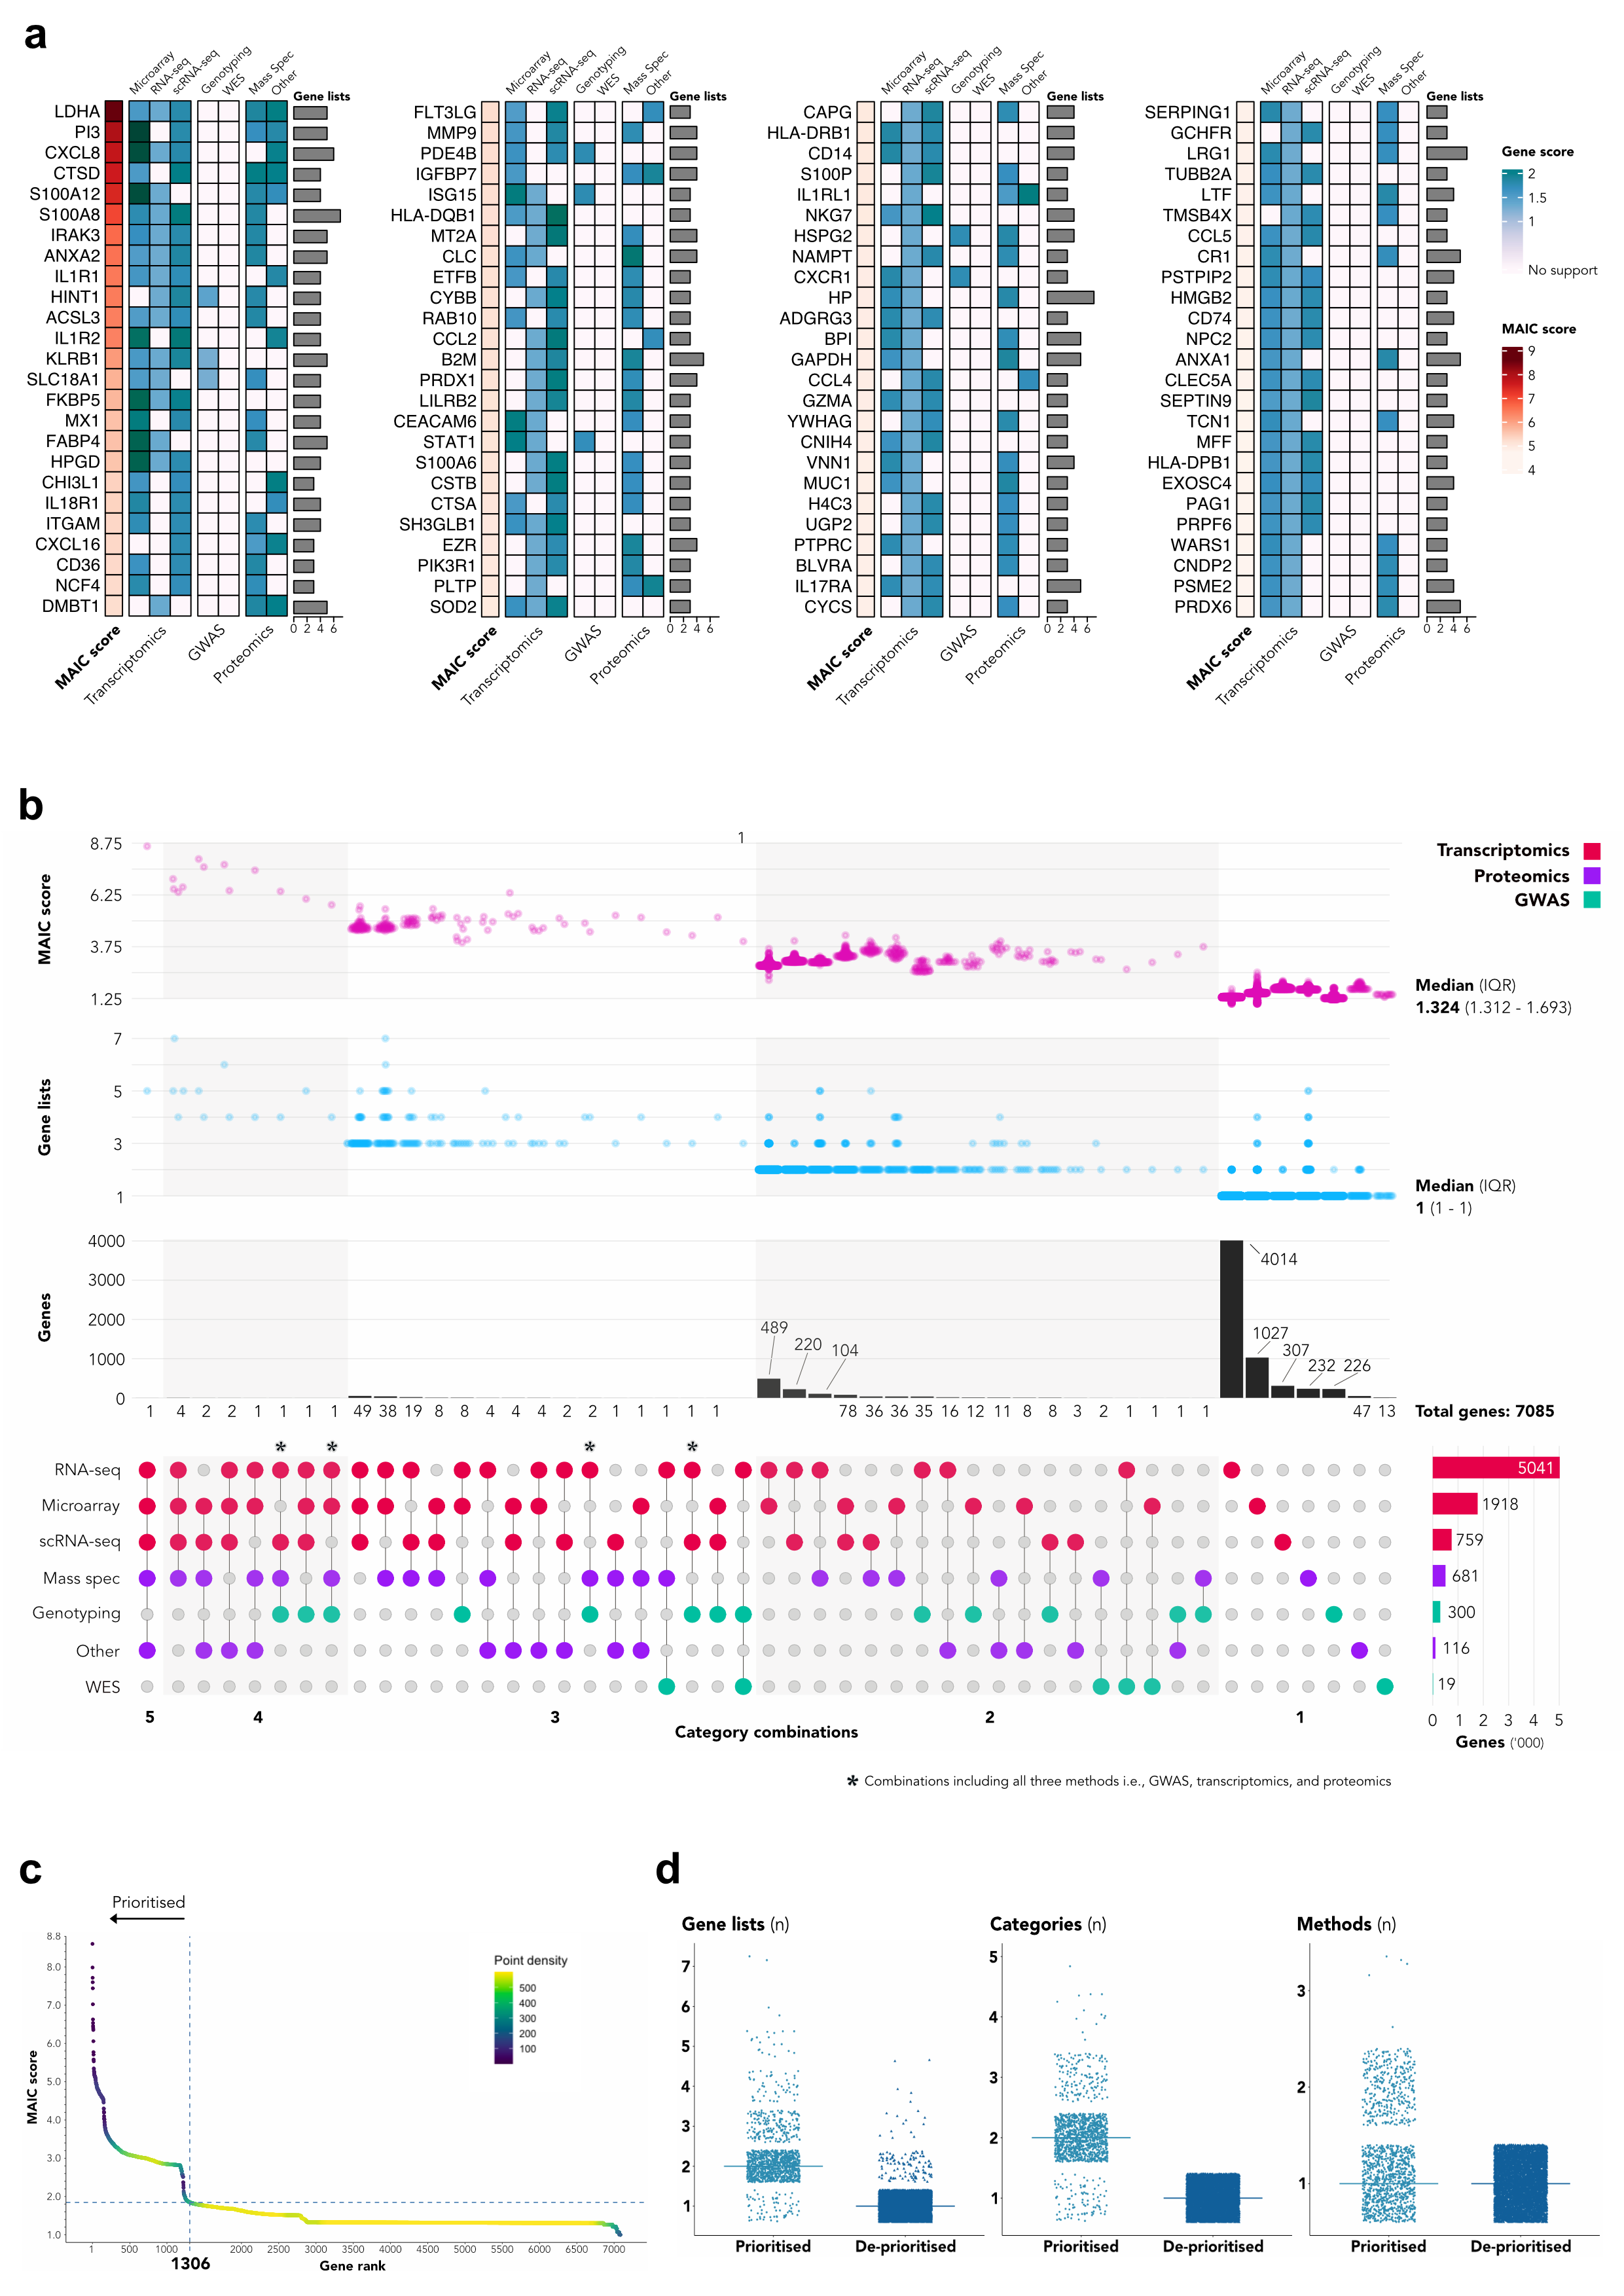
\includegraphics{./img/Figure_1.png}

}

\caption{\label{fig-fig1}\textbf{Meta-analysis by information content}.
(a) Heatmap of top 100 ranked genes showing MAIC score, highest score
per category, and number of supporting lists. (b) UpSet plot of MAIC
genes showing total numbers for each category combination, MAIC score
distribution, and supporting lists. (b) Gene prioritization using the
Unit Invariant Knee method. Intersection of lines identifies elbow point
of best-fit curve. 1,306 genes in upper left quadrant were prioritied.
(c) Strip plots comparing number of lists and categories/methods per
gene between prioritized and deprioritized sets.}

\end{figure}

To assess the influence of individual lists, we calculated the
information content (IC), reflecting the sum of gene scores across all
lists (Figure~\ref{fig-fig2}), and the information contribution (ICtb),
measuring the sum of gene scores contributing to a gene's overall MAIC
score. To obtain relative values, we divided the IC/ICtb for each list
by the total. This demonstrated that only 10 lists (from 9 studies)
contributed \textgreater1\% of the total information by either metric
(Tab. S2). Notably, the RNA-seq list from Sarma et
al.\textsuperscript{10} accounts for \textgreater50\% of the total IC
and ICtb, a function of its length. To account for this, we normalised
relative IC/ICtb by the number of genes per list. Along with the
proportion of replicated genes in each list, this provides an
alternative perspective, with several proteomic studies ranking highly
(Figure~\ref{fig-fig2}).

\begin{figure}

{\centering 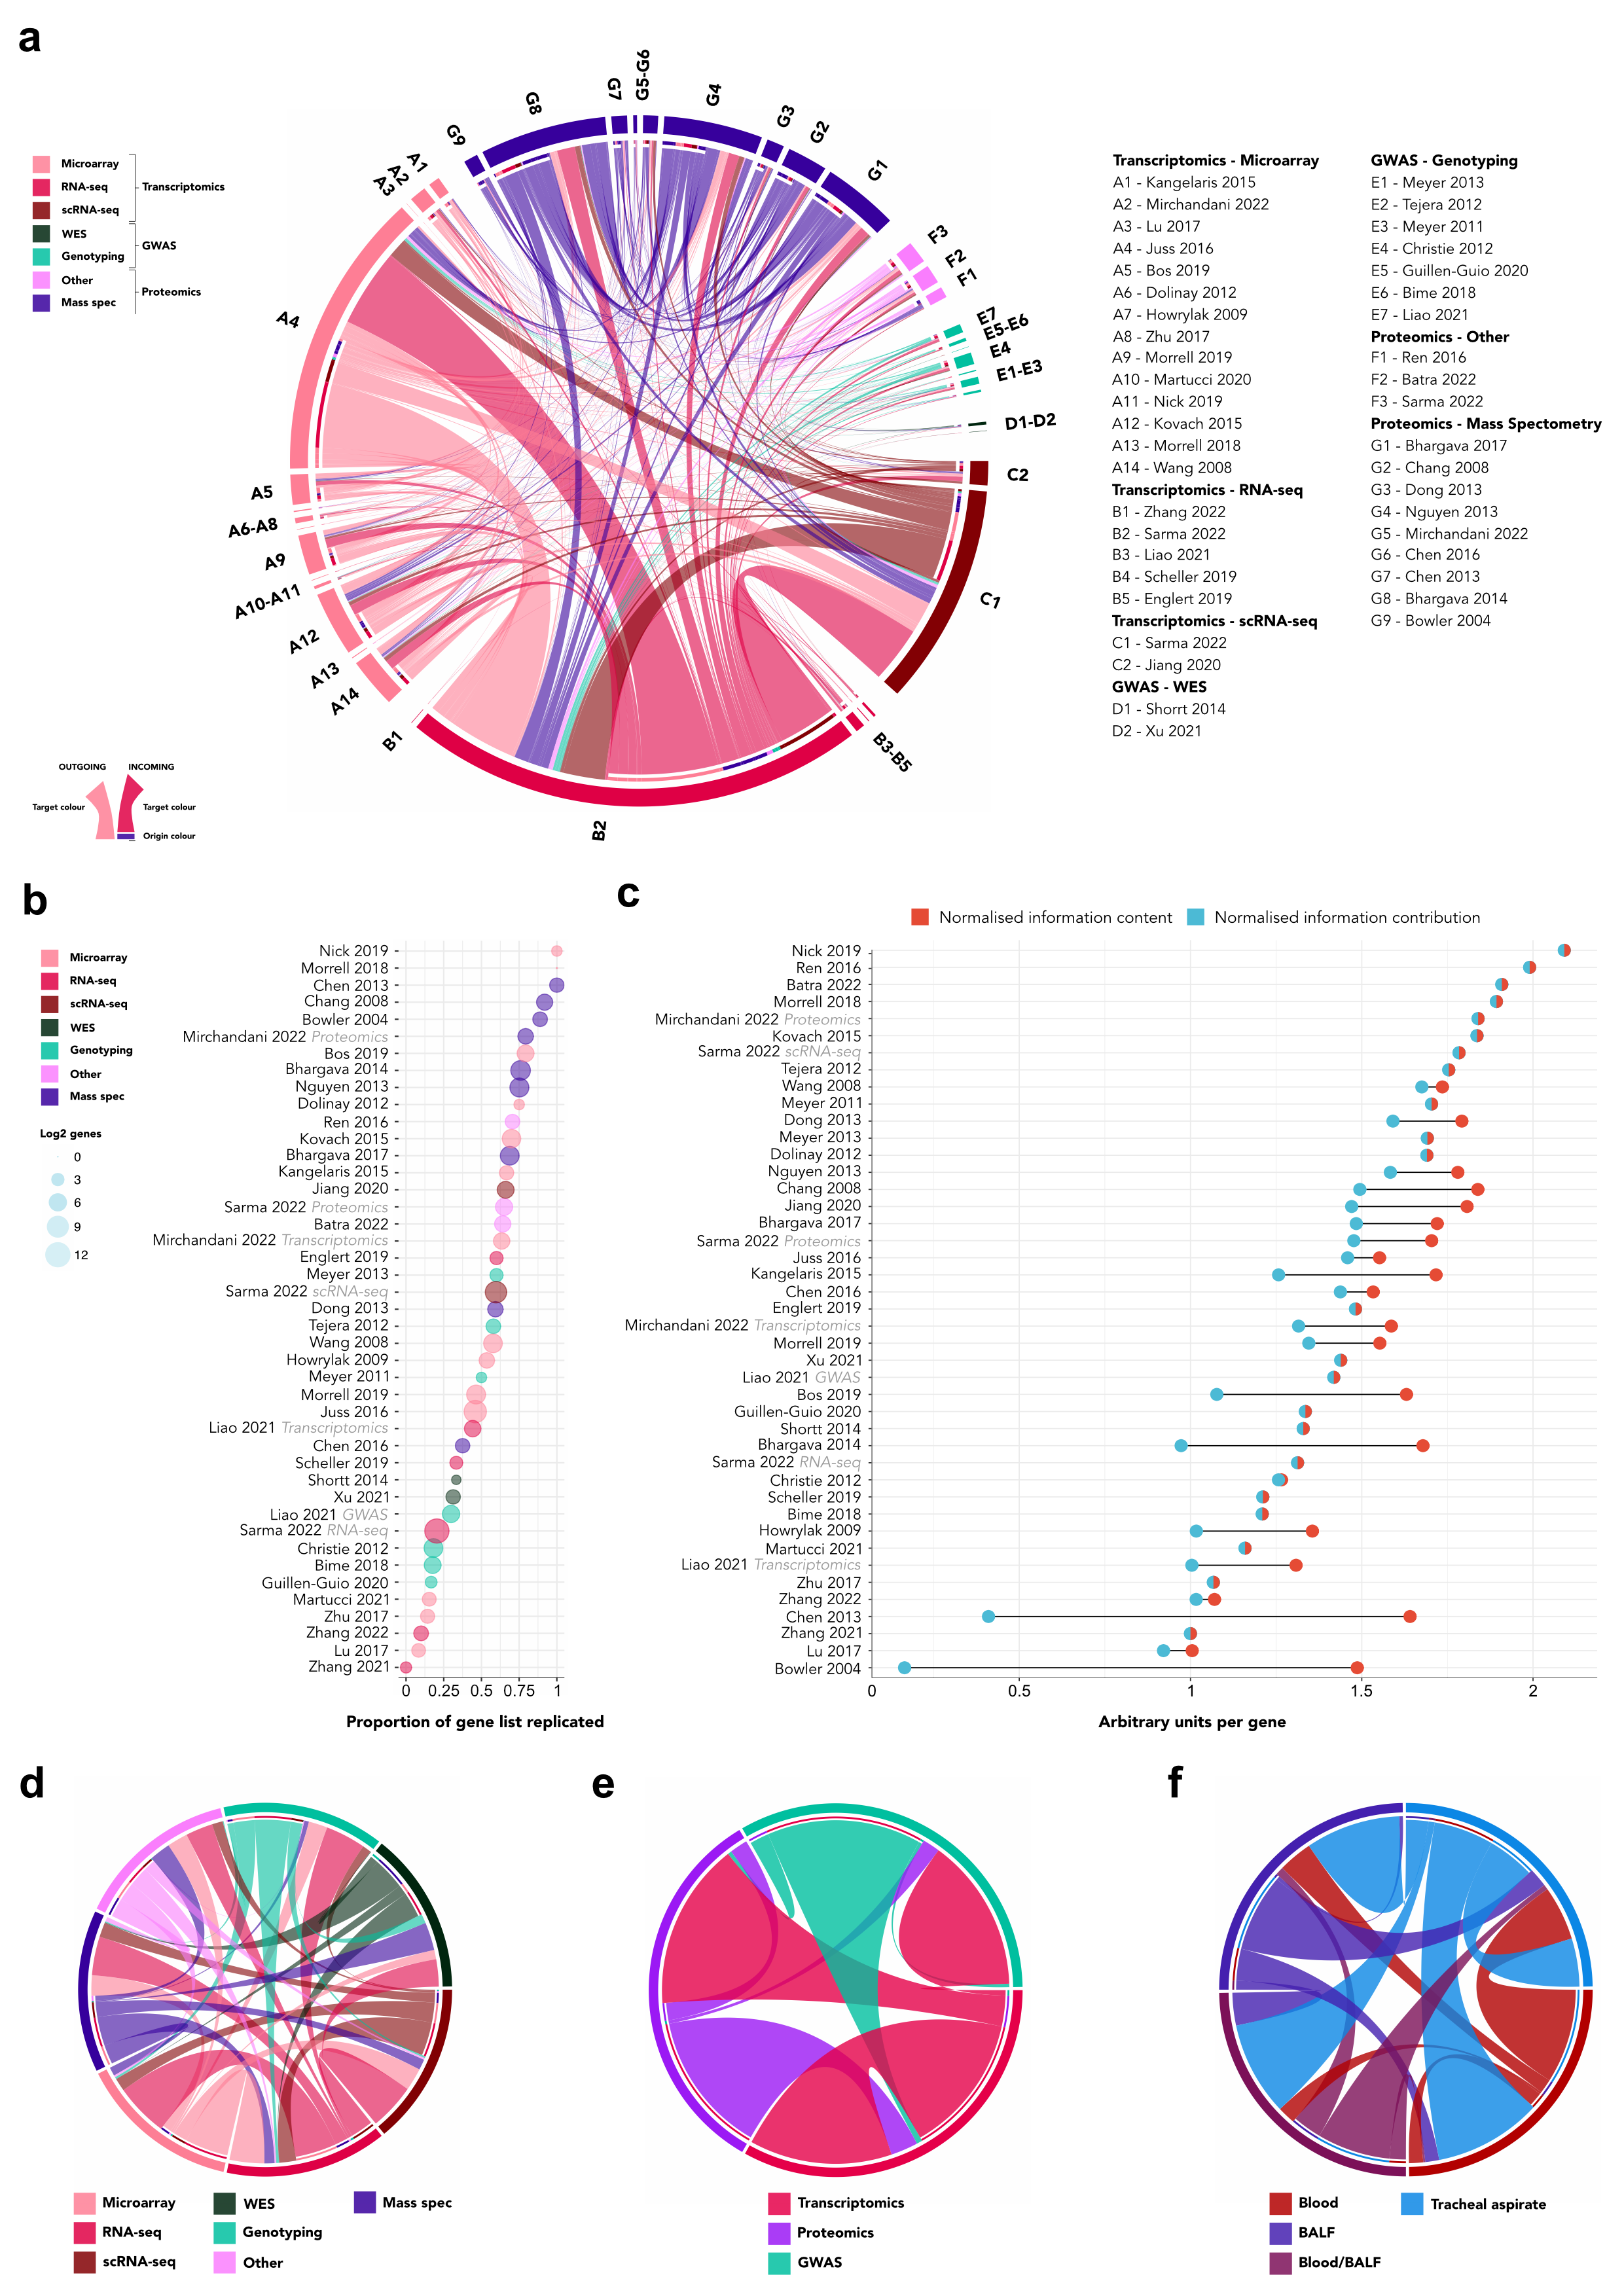
\includegraphics{./img/Figure_2.png}

}

\caption{\label{fig-fig2}\textbf{Attributing information in MAIC}. (a)
Shared information content (IC) between gene lists. Links indicate
absolute IC (sum of common gene scores) between studies. (b) Proportion
of replicated genes. Circle diameter is logarithm (base 2) of gene
number per list. (c) IC normalized by number of genes. Overlapping
circles denote equal normalized IC and contribution (ICtb - sum of
common gene scores contributing to MAIC), indicating all gene scores
contributed to MAIC. (d) Shared IC between categories, scaled so links
show fraction of total IC. (e) Shared IC between methods, scaled. (f)
Shared IC between tissue types, scaled.}

\end{figure}

\hypertarget{comparison-with-existing-ards-sources-and-covid-19}{%
\paragraph{Comparison with existing ARDS sources and
COVID-19}\label{comparison-with-existing-ards-sources-and-covid-19}}

To place our meta-analysis results in context, we evaluated the overlap
between the genes prioritised by MAIC and those from two established
resources: BioLitMine\textsuperscript{54}, using an ARDS MeSH search,
and the ARDS Database of Genes\textsuperscript{55} (Fig. S2a and Fig.
S2c). BioLitMine identified 271 ARDS-associated genes, of which 142
(52.4\%) were present in our analysis. Almost half of the overlapping
genes (n = 63, 44.4\%) ranked within our prioritised set (Tab. S3). Of
the 239 genes catalogued in the ARDS Database of Genes, 177 (74.1\%)
were also found in our study. However, both sources contain gene
associations lacking genome-wide support.

\newpage

\blandscape

\hypertarget{tbl-tab1}{}
\begin{longtable}[]{@{}
  >{\raggedright\arraybackslash}p{(\columnwidth - 16\tabcolsep) * \real{0.0694}}
  >{\raggedright\arraybackslash}p{(\columnwidth - 16\tabcolsep) * \real{0.2222}}
  >{\raggedright\arraybackslash}p{(\columnwidth - 16\tabcolsep) * \real{0.1111}}
  >{\raggedright\arraybackslash}p{(\columnwidth - 16\tabcolsep) * \real{0.1111}}
  >{\raggedright\arraybackslash}p{(\columnwidth - 16\tabcolsep) * \real{0.0694}}
  >{\raggedright\arraybackslash}p{(\columnwidth - 16\tabcolsep) * \real{0.1181}}
  >{\raggedright\arraybackslash}p{(\columnwidth - 16\tabcolsep) * \real{0.1111}}
  >{\raggedright\arraybackslash}p{(\columnwidth - 16\tabcolsep) * \real{0.0833}}
  >{\raggedright\arraybackslash}p{(\columnwidth - 16\tabcolsep) * \real{0.1042}}@{}}
\caption{\label{tbl-tab1}Summary of studies and gene lists included in
the systematic review}\tabularnewline
\toprule\noalign{}
\begin{minipage}[b]{\linewidth}\raggedright
\textbf{Year}
\end{minipage} & \begin{minipage}[b]{\linewidth}\raggedright
\textbf{Study}
\end{minipage} & \begin{minipage}[b]{\linewidth}\raggedright
\textbf{Focus}
\end{minipage} & \begin{minipage}[b]{\linewidth}\raggedright
\textbf{Definition}
\end{minipage} & \begin{minipage}[b]{\linewidth}\raggedright
\textbf{N}\textsuperscript{a}
\end{minipage} & \begin{minipage}[b]{\linewidth}\raggedright
\textbf{Method}
\end{minipage} & \begin{minipage}[b]{\linewidth}\raggedright
\textbf{Technique}
\end{minipage} & \begin{minipage}[b]{\linewidth}\raggedright
\textbf{Tissue}
\end{minipage} & \begin{minipage}[b]{\linewidth}\raggedright
\textbf{Cell type}
\end{minipage} \\
\midrule\noalign{}
\endfirsthead
\toprule\noalign{}
\begin{minipage}[b]{\linewidth}\raggedright
\textbf{Year}
\end{minipage} & \begin{minipage}[b]{\linewidth}\raggedright
\textbf{Study}
\end{minipage} & \begin{minipage}[b]{\linewidth}\raggedright
\textbf{Focus}
\end{minipage} & \begin{minipage}[b]{\linewidth}\raggedright
\textbf{Definition}
\end{minipage} & \begin{minipage}[b]{\linewidth}\raggedright
\textbf{N}\textsuperscript{a}
\end{minipage} & \begin{minipage}[b]{\linewidth}\raggedright
\textbf{Method}
\end{minipage} & \begin{minipage}[b]{\linewidth}\raggedright
\textbf{Technique}
\end{minipage} & \begin{minipage}[b]{\linewidth}\raggedright
\textbf{Tissue}
\end{minipage} & \begin{minipage}[b]{\linewidth}\raggedright
\textbf{Cell type}
\end{minipage} \\
\midrule\noalign{}
\endhead
\bottomrule\noalign{}
\endlastfoot
2022 & Batra\textsuperscript{15} & Survival & Berlin & 24 & Proteomics &
Other & Blood & \\
& Mirchandani\textsuperscript{39} & Susceptibility & Berlin & 22 &
Proteomics & Mass Spec & Blood & Monocytes \\
& & & & & Transcriptomics & Microarray & Blood & Monocytes \\
& Sarma\textsuperscript{10} & Sub-phenotype & Berlin & 41 & Proteomics &
Other & TA & \\
& & & & & Transcriptomics & RNA-seq & TA & \\
& & & & & Transcriptomics & scRNA-Seq & TA & Immune cells \\
& Zhang\textsuperscript{51} & Susceptibility & AECC & 11 &
Transcriptomics & RNA-Seq & Blood & Exosomes \\
2021 & Liao\textsuperscript{34} & Survival & Either & 390 & GWAS &
Genotyping & Blood & \\
& & & & & Transcriptomics & RNA-seq & Blood & PBMCs \\
& Martucci\textsuperscript{36} & Sub-phenotype & None & 11 &
Transcriptomics & Microarray & Blood & \\
& Xu\textsuperscript{49} & Survival & Berlin & 105 & GWAS & WES & Blood
& \\
& Zhang\textsuperscript{50} & Susceptibility & Berlin & 5 &
Transcriptomics & RNA-seq & Blood & \\
2020 & Guillen-Guio\textsuperscript{28} & Susceptibility & Berlin & 633
& GWAS & Genotyping & Blood & \\
& Jiang\textsuperscript{30} & Susceptibility & Berlin & 3 &
Transcriptomics & scRNA-seq & Blood & PBMCs \\
2019 & Bos\textsuperscript{9} & Sub-phenotype & Berlin & 210 &
Transcriptomics & Microarray & Blood & \\
& Englert\textsuperscript{26} & Susceptibility & Either & 11 &
Transcriptomics & RNA-seq & Blood & \\
& Morrell\textsuperscript{41} & Survival & AECC & 36 & Transcriptomics &
Microarray & BALF & AMs \\
& Scheller\textsuperscript{45} & Susceptibility & None & 6 &
Transcriptomics & RNA-seq & BALF & EVs \\
2018 & Bime\textsuperscript{18} & Susceptibility & Either & 232 & GWAS &
Genotyping & Blood & \\
& Morrell\textsuperscript{40} & Susceptibility & Berlin & 35 &
Transcriptomics & Microarray & BALF & \\
2017 & Bhargava\textsuperscript{17} & Survival & AECC & 36 & Proteomics
& Mass Spec & BALF & \\
& Lu\textsuperscript{35} & Susceptibility & AECC & 12 & Transcriptomics
& Microarray & Blood & \\
& Zhu\textsuperscript{52} & Susceptibility & Berlin & 199 &
Transcriptomics & Microarray & Blood & \\
2016 & Chen\textsuperscript{22} & Severity & AECC & 7 & Proteomics &
Mass Spec & BALF/Blood & \\
& Juss\textsuperscript{31} & Susceptibility & Berlin & 23 &
Transcriptomics & Microarray & Blood & Neutrophils \\
& Nick\textsuperscript{42} & Sub-phenotype & AECC & 121 &
Transcriptomics & Microarray & Blood & Neutrophils \\
& Ren\textsuperscript{44} & Susceptibility & Berlin & 14 & Proteomics &
Other & Blood & \\
2015 & Kangelaris\textsuperscript{32} & Susceptibility & Berlin & 29 &
Transcriptomics & Microarray & Blood & \\
& Kovach\textsuperscript{33} & Susceptibility & AECC & 18 &
Transcriptomics & Microarray & BALF/Blood & AMs \\
2014 & Bhargava\textsuperscript{16} & Progression & AECC & 22 &
Proteomics & Mass Spec & BALF & \\
& Shortt\textsuperscript{46} & Susceptibility & AECC & 213 & GWAS & WES
& Blood & \\
2013 & Chen\textsuperscript{21} & Susceptibility & Berlin & 11 &
Proteomics & Mass Spec & Blood & \\
& Dong\textsuperscript{25} & Progression & None & 14 & Proteomics & Mass
Spec & BALF & AMs \\
& Meyer\textsuperscript{38} & Susceptibility & Berlin & 661 & GWAS &
Genotyping & Blood & \\
& Nguyen\textsuperscript{43} & Susceptibility & AECC & 30 & Proteomics &
Mass Spec & BALF & \\
2012 & Christie\textsuperscript{23} & Susceptibility & AECC & 812 & GWAS
& Genotyping & Blood & \\
& Dolinay\textsuperscript{24} & Susceptibility & AECC & 35 &
Transcriptomics & Microarray & Blood & \\
& Tejera\textsuperscript{48} & Susceptibility & AECC & 1400 & GWAS &
Genotyping & Blood & \\
2011 & Frenzel\textsuperscript{27} & Survival & AECC & 46 & Proteomics &
Mass Spec & BALF & \\
& Meyer\textsuperscript{37} & Susceptibility & AECC & 1241 & GWAS &
Genotyping & Blood & \\
2009 & Howrylak\textsuperscript{29} & Susceptibility & AECC & 13 &
Transcriptomics & Microarray & Blood & \\
2008 & Chang\textsuperscript{20} & Susceptibility & None & 20 &
Proteomics & Mass Spec & BALF & \\
& Wang\textsuperscript{47} & Susceptibility & AECC & 8 & Transcriptomics
& Microarray & Blood & \\
2004 & Bowler\textsuperscript{19} & Susceptibility & AECC & 16 &
Proteomics & Mass Spec & BALF/Blood & \\
\end{longtable}

\begin{scriptsize}
a - The number of patients with ARDS included in each study.
Abbreviations: AECC - American-European Consensus Conference; AMs - Alveolar macrophages; BALF - Bronchoalveolar lavage fluid; EVs - Extracellular vesicles; GWAS - Genome-wide association study; MS - Mass spectometry; PBMCs - Peripheral blood mononuclear cells; TA - Tracheal aspirate; WES - Whole-exome sequencing. 
\end{scriptsize}

\elandscape

\newpage

After correcting historical gene symbol aliases, we matched 4 additional
genes from the BioLitMine search not initially found in the ARDS MAIC
set. A further 104 genes from this search were supported by just a
single publication (Fig S2b). For each of the remaining 21 genes, we
obtained the 100 most co-expressed genes using
ARCHS4\textsuperscript{56} (returning data for 18) and assessed the
overlap of these sets with ARDS MAIC; two-thirds exhibited \textless50\%
overlap (Fig. S2b). Finally, we compared the overlap between genes
ranked by ARDS MAIC and those identified in a previous MAIC of the host
response to COVID-19\textsuperscript{13} (Fig. S2d). In total, 2,606
ARDS-associated genes (36.8\%) were common to both analyses, of which
143 were prioritised by both (Fig. S2e).

\hypertarget{tissue-and-cell-specific-expression}{%
\paragraph{Tissue and cell-specific
expression}\label{tissue-and-cell-specific-expression}}

Although most gene lists were derived from blood sampling, most genes
were identified in airway samples (n=5,847, 82.5\%) (Fig. S3a). This was
also true for the prioritized gene set, however most of these were also
identified in blood (n=818, 62.6\%) (Fig. S3b). For the genes uniquely
identified in lists from blood samples (n=1,238), almost three-quarters
are known to be expressed in the lung (HPA scRNA-seq data, ≥ 5
normalised transcripts per million (nTPM)), with a quarter being
highly-expressed (≥ 100 nTPM) (Fig. S3c). For prioritized lung genes,
there is a wide variety of cell-specific expression (Fig. S3d). However,
in the smaller set of prioritized genes identified only in blood,
clusters of expression specific to neutrophils, T cells, and monocytes
are evident (Fig. S3e). Cell-type specific gene enrichment analysis
suggests innate immune as well as epithelial and endothelial cell types
are enriched among genes identified in airway samples (Fig. S3f).
However, enrichment of epithelial and endothelial cells is not evident
for prioritized genes identified from blood sampling alone (Fig. S3g).

\hypertarget{functional-enrichment}{%
\paragraph{Functional enrichment}\label{functional-enrichment}}

Having identified a set of prioritised genes, we undertook several
functional enrichment analyses. First, we performed over-representation
analysis (ORA). In Reactome, 51 terms were significantly enriched
(\emph{P} \textless{} 0.001) (Figure~\ref{fig-fig3}). As expected,
neutrophil degranulation and several innate immune pathways (e.g., IL-10
signalling, interferon signalling, MHC II antigen presentation, TLR4
cascade) feature heavily. However, multiple pathways associated with
cholesterol biology and metabolism (e.g., chylomicron
assembly/remodelling, GLUT4 translocation, TP53 regulation of metabolic
genes, insulin regulation) were also over-represented. Similarly, lipid
and cholesterol metabolism, as well as hyperlipidaemia, were
over-represented in KEGG and WikiPathways (Fig. S4a and Fig. S4b). In an
enrichment analysis using the GWAS Catolog, the prioritised set of genes
was associated with asthma (adult onset/time to onset), monocyte,
lymphocyte, and eosinophil counts, aspartate aminotransferase levels,
and levels of apolipoprotein A1 (Fig. S4d).

Next, we used the prioritised set of genes to create a protein-protein
interaction (PPI) network. We graph-clustered this network, identifying
48 clusters with ≥ 5 members. Among the 10 largest clusters, we found
programs associated with the proteaosome, cholesterol metabolism,
interferon signalling, IL-6 signalling, and the complement cascade (Fig.
S5). We then sought to use the PPI network to identify hub genes using
an ensemble of topological methods. This analysis suggested 51 genes
central to the wider network (Figure~\ref{fig-fig3}). Clustering these
genes alone identified 5 clusters, which may be associated with innate
immune cytokine signalling, interferon signalling, MHC class II antigen
presentation, PI3K-Akt signalling, and eukaryotic translation elongation
(Figure~\ref{fig-fig3}). The majority of hub genes (n=31, 61\%) are
currently druggable and include targets such as \emph{IL-6},
\emph{IL-17A}, \emph{IL-18}, and \emph{MAP3K14}.

\begin{figure}

{\centering 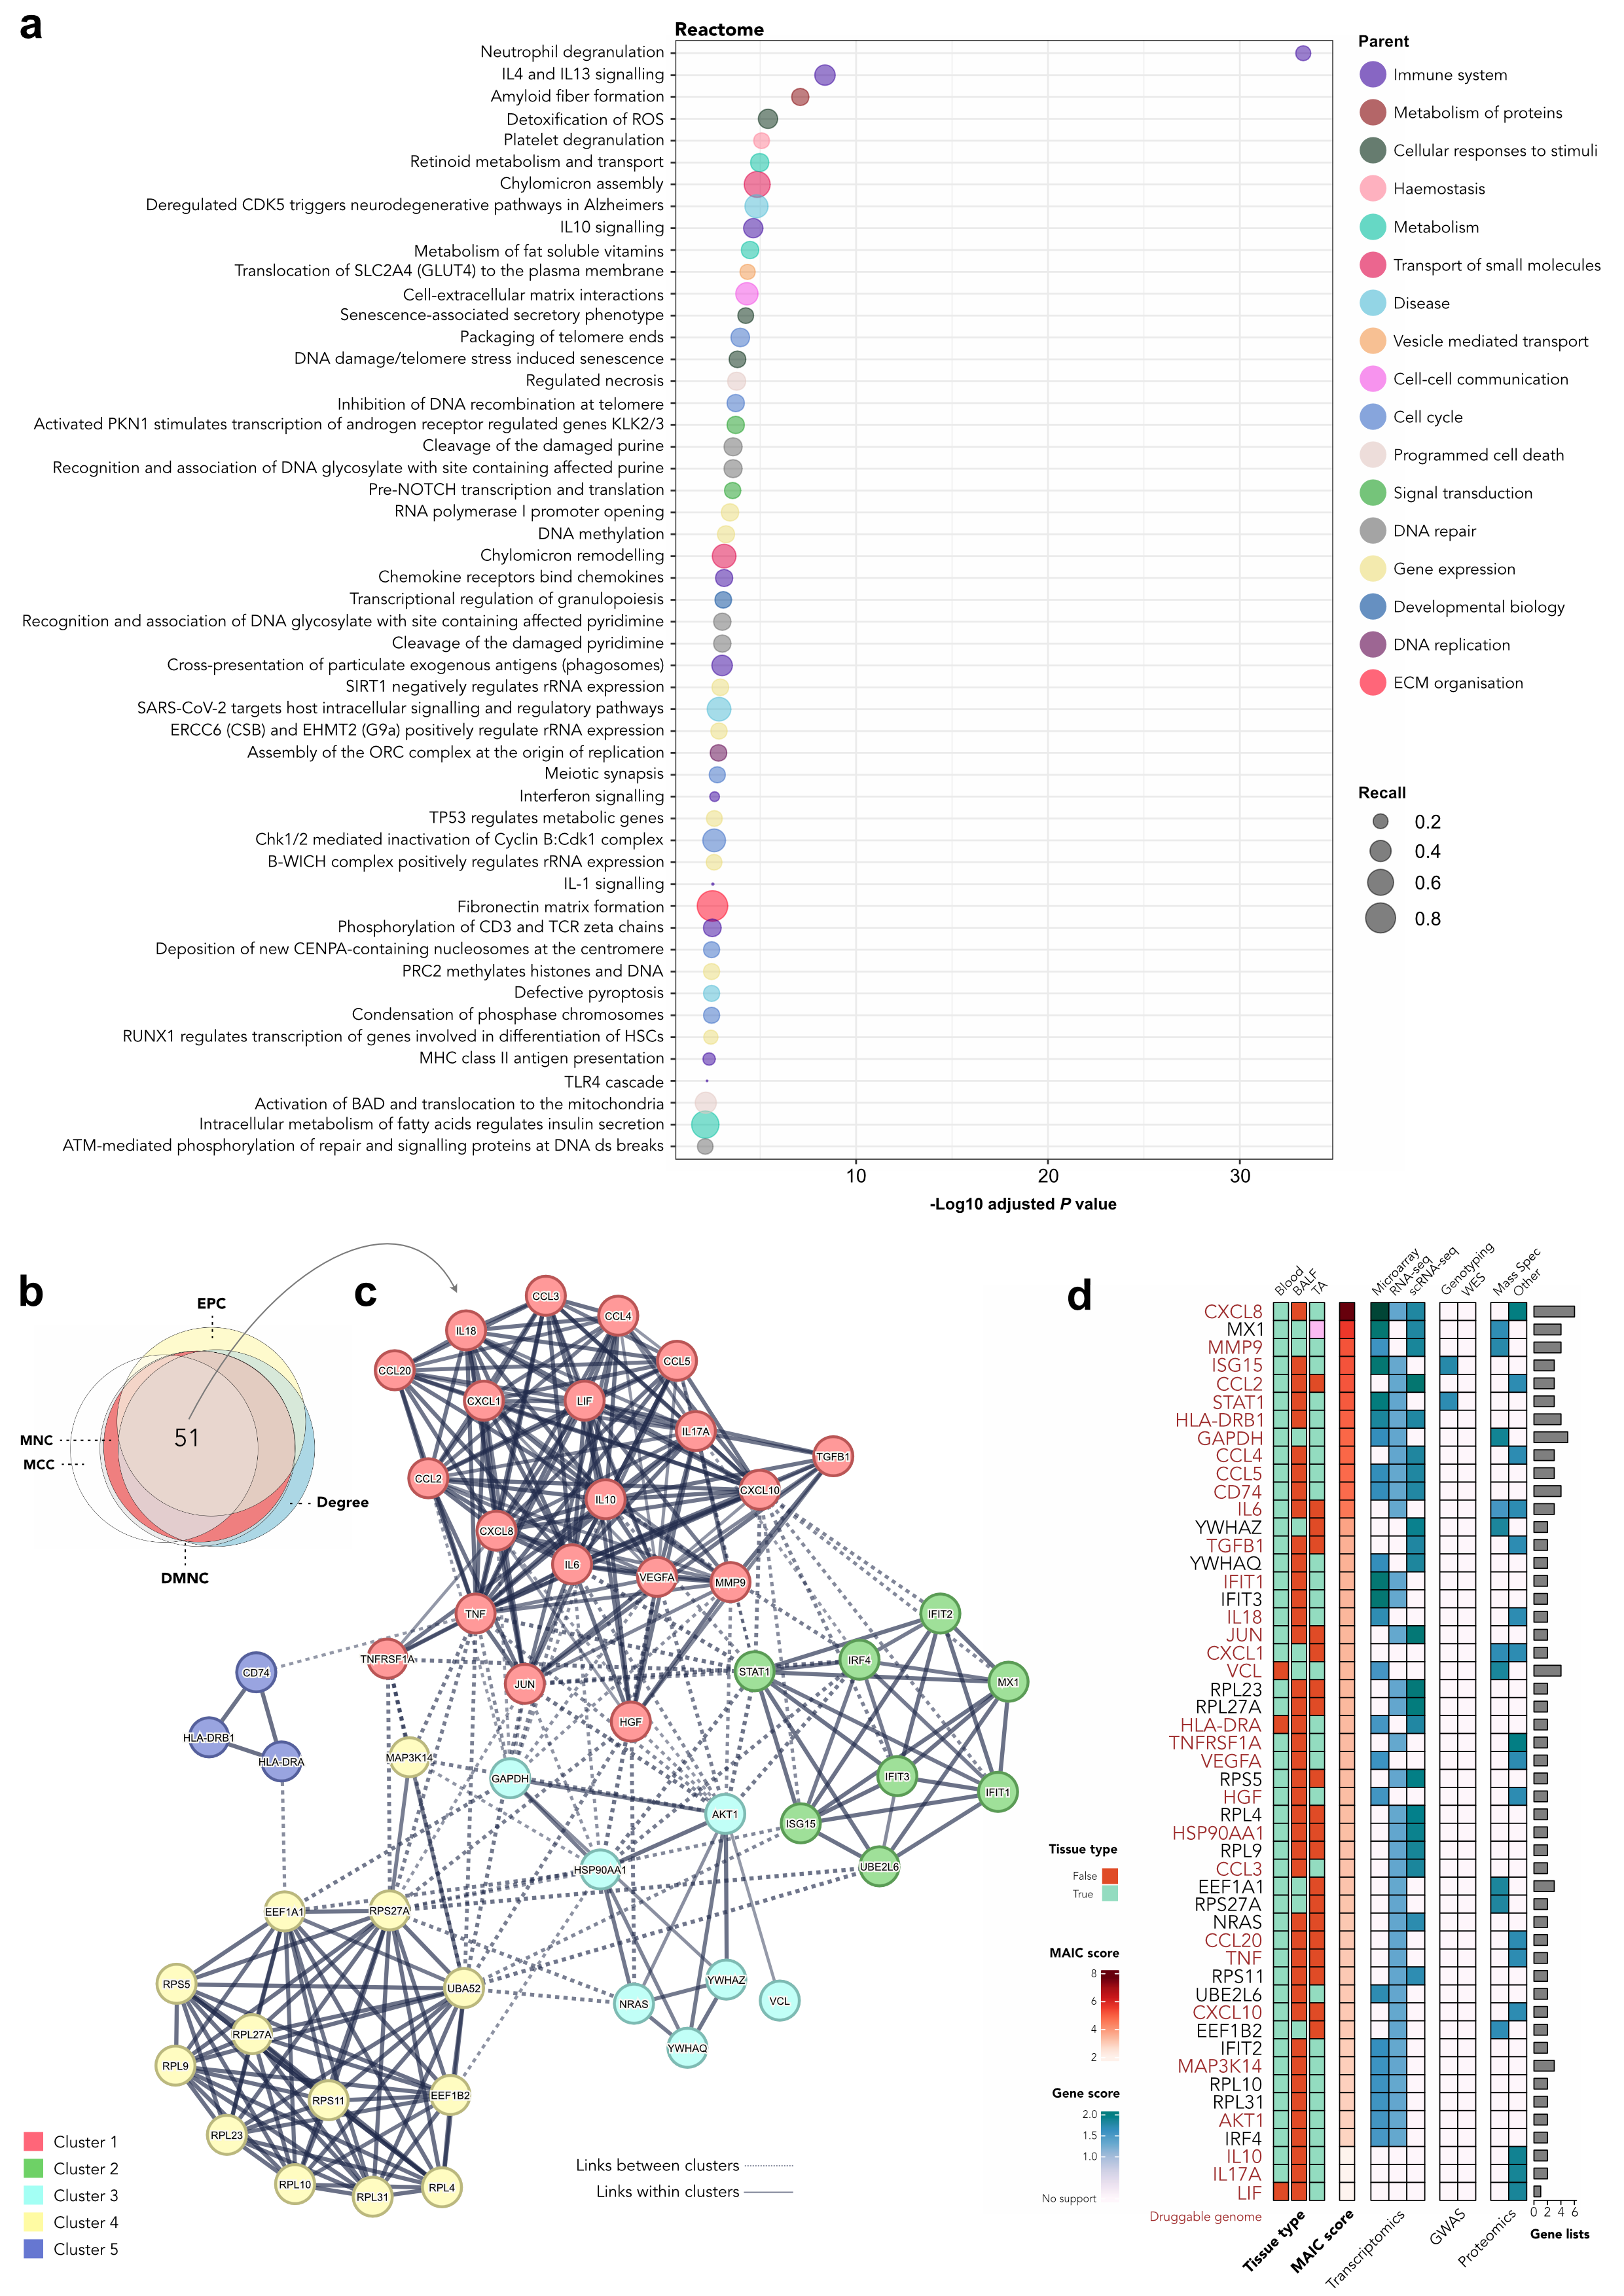
\includegraphics{./img/Figure_3.png}

}

\caption{\label{fig-fig3}\textbf{Functional enrichment of prioritised
genes}. (a) Significantly enriched Reactome terms (\emph{P} \textless{}
0.01). Terms colored by parent class and size proportional to recall.
(b) Euler diagram of the overlap of hub genes identified by five
methods. MNC - Maximum Neighbourhood Component, MCC - Maximal Clique
Centrality, DMNC - Density of MNC, EPC - Edge Percolated Component. (c)
Protein-protein interaction (PPI) network of hub genes, clustered using
the Markov Chain Algorithm. (d). Heatmap of common hub genes displaying
tissue type(s), MAIC score, highest category score, supporting lists,
and presence in the druggable genome.}

\end{figure}

\hypertarget{sub-groups}{%
\paragraph{Sub-groups}\label{sub-groups}}

A source of tension in our approach is the balance between dispartiy in
study designs (e.g., susceptibilty, sub-phenotype) and the requirement
for sufficient data to make meaningful inferences. To address this, we
undertook MAIC on subsets of gene lists, stratified by study focus.
There were sufficient lists to make this tractable for studies focused
on susceptibility to ARDS (n=28) and studies of ARDS survival and
severity (n=7) (Figure~\ref{fig-fig4}).

For susceptibility, there were 15 transcriptomic (54\%), 7 GWAS (25\%),
and 6 proteomic lists (21\%). MAIC ranked 2,096 genes
(Figure~\ref{fig-fig4}). The majority of these (n=1,222, 58\%) were
unique to susceptibility-based lists (Figure~\ref{fig-fig4}). Most were
identified in blood, with a small fraction found solely in airways
samples. The inflection point method prioritised the top ranked 130
genes (Fig. S6a). In comparison to the BioLitMine search and the ARDS
Database of Genes, 71/271 and 117/239 genes were found among the ARDS
MAIC susceptibility set respectively (Fig. S6b). A microarray-based
transcriptomic list from Juss \emph{et. al.}\textsuperscript{31}
accounted for more than half (54.7\%) of the relative ICtb, with an
additional 12 lists having a relative ICtb ≥ 1\% (Tab. S4). ORA using
Reactome, KEGG, and WikiPathways identified 25 significantly enriched
pathways including multiple terms related to cholesterol metabolism and
glycolysis (Fig. S7a). A consensus of topological models identified 7
hub genes within a PPI network of prioritised genes. These genes cluster
in a single group, characterised as being related to cholesterol
metabolism by several pathway databases (Figure~\ref{fig-fig4}).

For survival, the 8 gene lists consisted of 3 transcriptomic lists
(37.5\%), 3 proteomic lists (37.5\%), and 2 GWAS (25\%). MAIC ranked 463
genes (Figure~\ref{fig-fig4}). Approximately half of these (n=238, 51\%)
were unique to survival-based lists. In contrast to the susceptibility
analysis, most survival genes were found in airways samples.
Thirty-three genes were prioritised (Fig. S6d). In total, 32/271 of the
BioLitMine ARDS-associated genes and 23/239 of the ARDS Database of
Genes genes were found among the ARDS MAIC survival set (Fig. S6e). The
proteomic and transcriptomic lists from Bhargava
\emph{et.al}\textsuperscript{17} and Morrell \emph{et.
al}\textsuperscript{41} each contributed approximately 30\% of the
relative ICtb (Tab. S5). IL-10 and IL-18 signalling pathways were both
significantly enriched in ORA (Fig. S7c). Graph-based clustering of the
prioritised set of survival genes identified a single large cluster of
immune-related genes including, \emph{IL-10}, \emph{CXCL8},
\emph{TNFRSF1A}, and \emph{IL2RA} (Fig. S7d).

\begin{figure}

{\centering 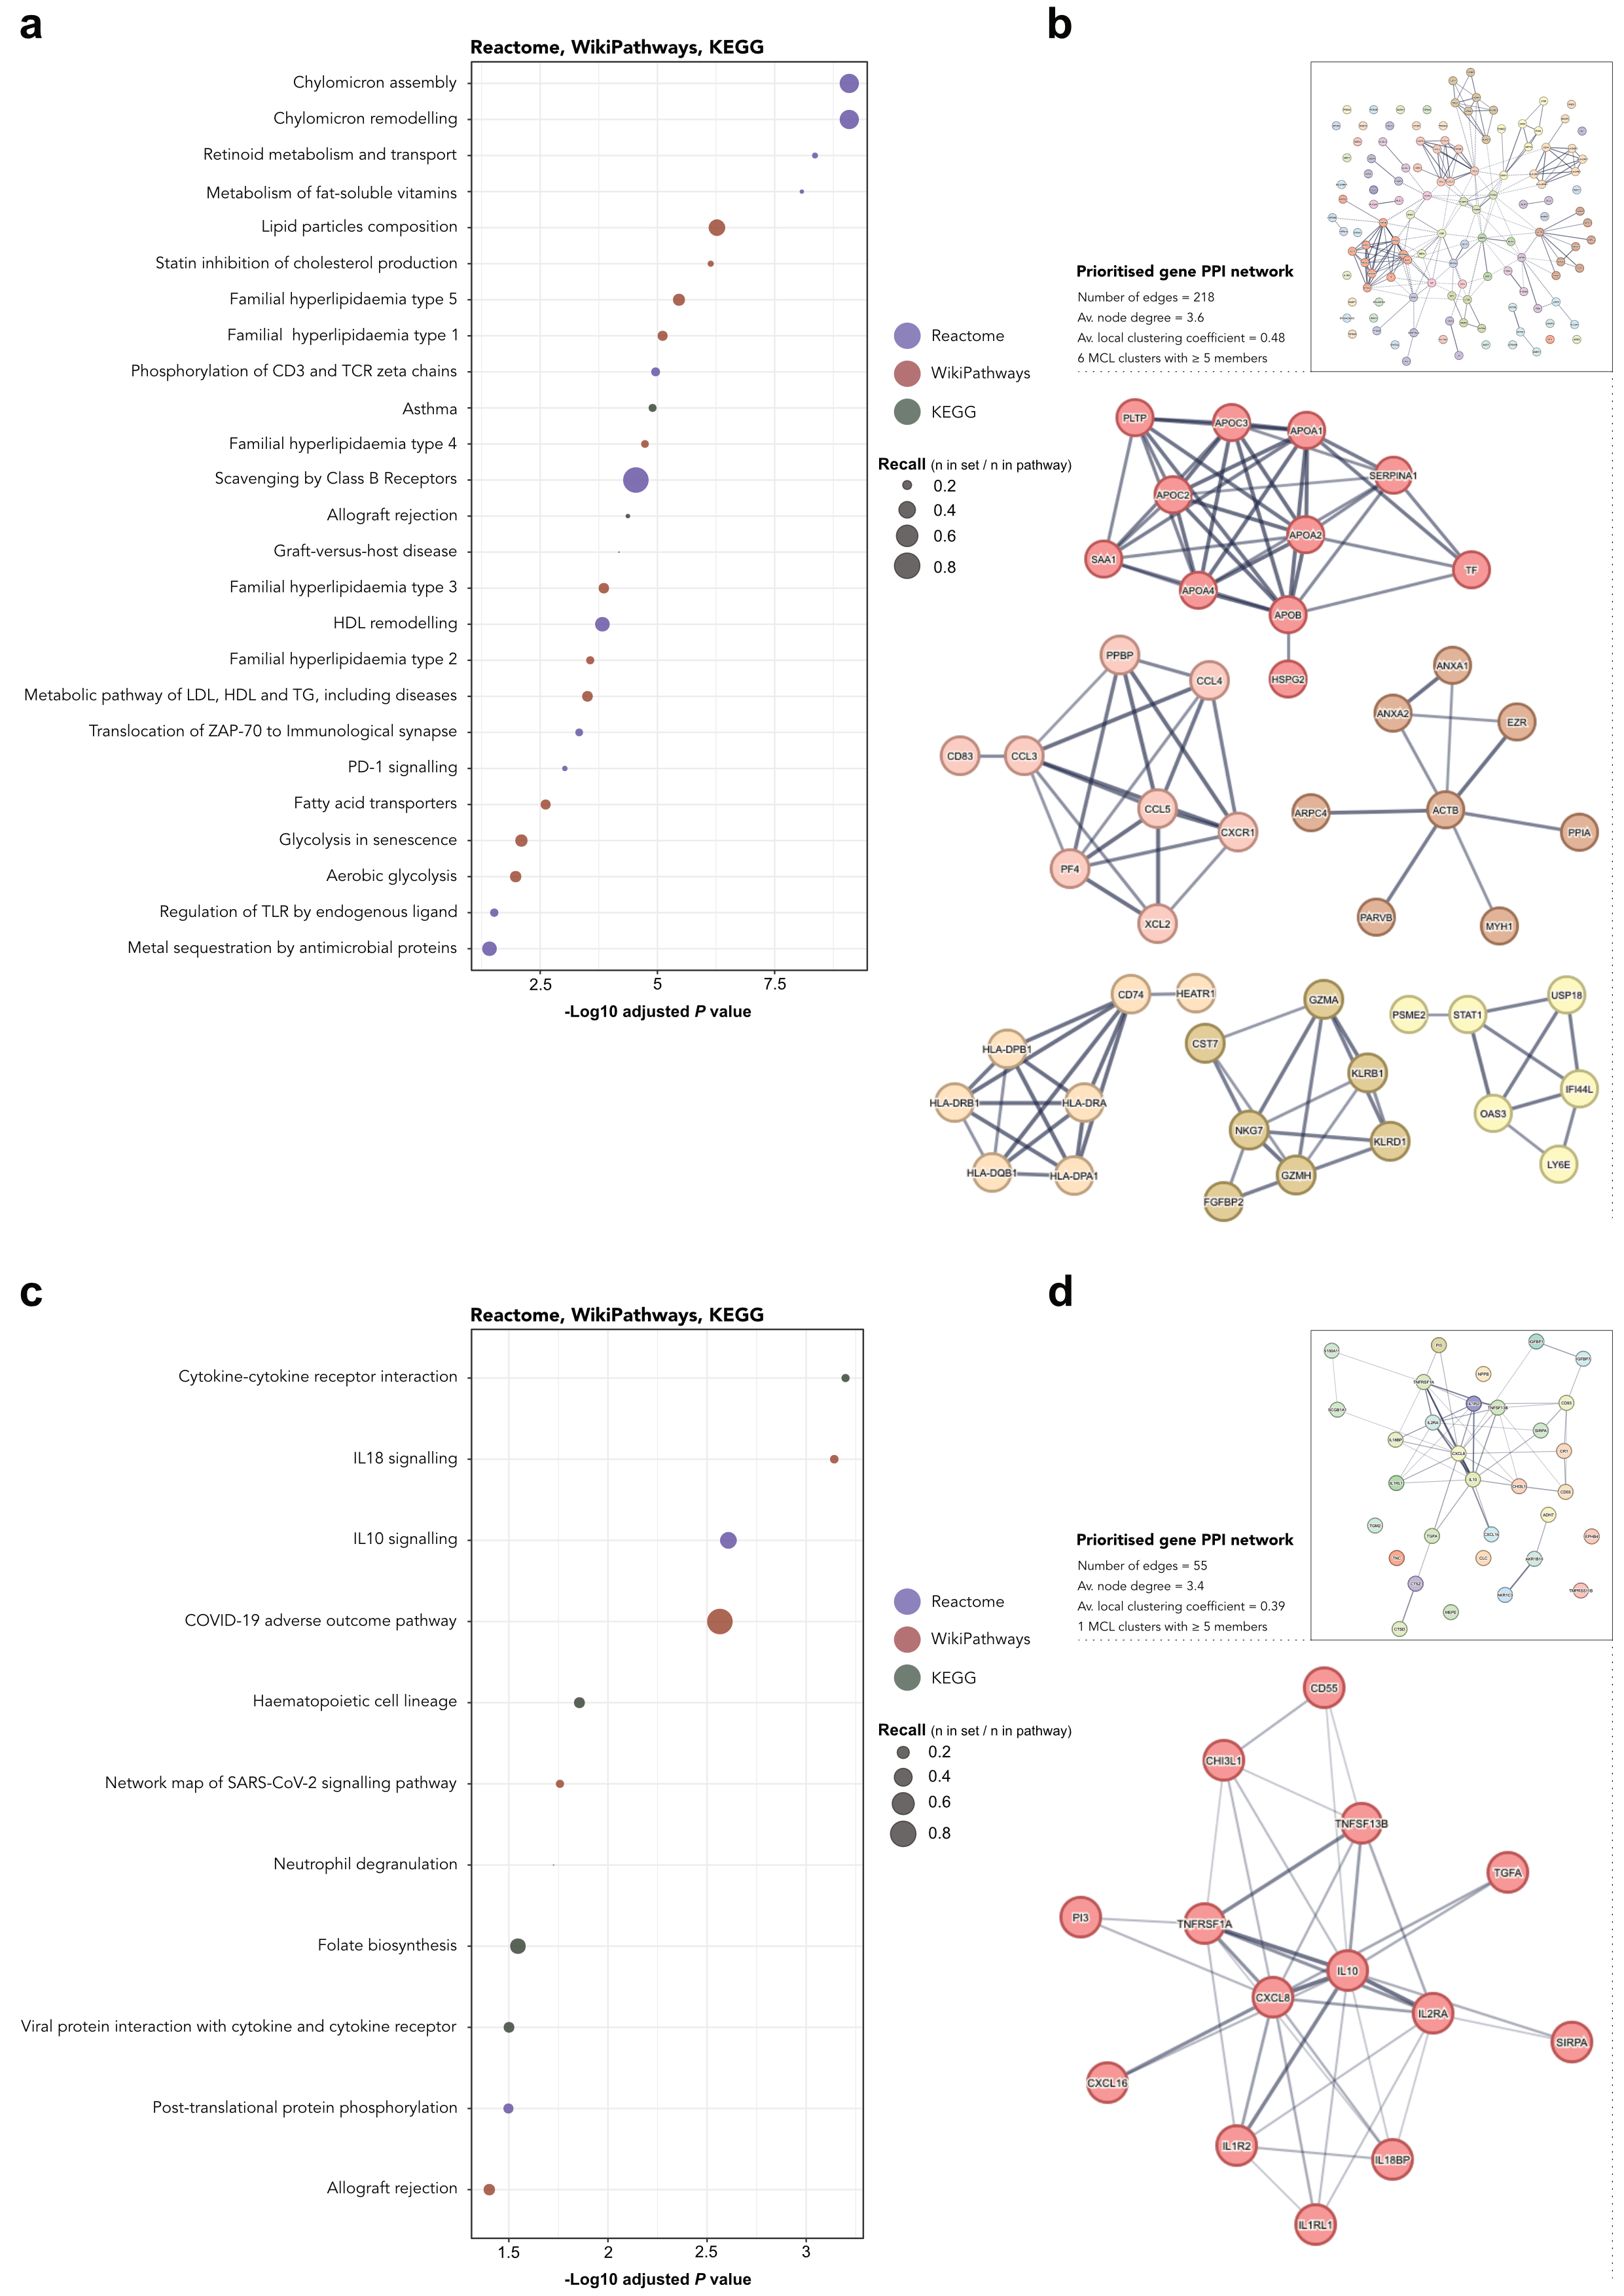
\includegraphics{./img/Figure_4.png}

}

\caption{\label{fig-fig4}\textbf{MAIC of sub-groups}. (a) Schematic of
ARDS MAIC sub-group analyses. (b) Heatmap of top 50 ranked genes in the
susceptibility set showing MAIC score, highest score per category, and
number of supporting lists. (c) Heatmap of 16 ranked genes in the
survival set with multi-list support showing MAIC score, highest score
per category, and number of supporting lists. (d) Eular diagram of gene
overlap between the susceptibility and survival sets and the remainder
of genes. (e) Bar plots of the tissue type in which genes are
identified. (f) plot comparing the ranks of susceptibility and survival
prioritised genes with their ranks in the full iteration of ARDS MAIC.
(g) Euler diagram of the overlap of hub genes identified by five
methods. MNC - Maximum Neighbourhood Component, MCC - Maximal Clique
Centrality, DMNC - Density of MNC, EPC - Edge Percolated Component and a
protein-protein interaction (PPI) network of hub genes, clustered using
the Markov Chain Algorithm - for susceptibility.}

\end{figure}

\newpage

\hypertarget{discussion}{%
\subsection{Discussion}\label{discussion}}

Our systematic integration and re-analysis of more than 20 years of data
is the first large-scale meta-analysis of the genomic landscape of ARDS.
This implicates over 7,000 genes and prioritises 1,306. The wide
inclusion criteria capture a diverse range of study designs and methods;
the subsequent application of MAIC establishes the sum of this
knowledge, downgrading noisy, irrelevant, or low-quality information.
These results have three main applications. First, they can be used to
better understand the pathobiology of ARDS, providing a resource to
prioritise future \emph{in-vitro} and \emph{in-vivo} studies and
permitting comparisons between important sub-groups. Second, they
prioritise therapeutic targets, serving as a source against which novel
and repurposed treatments can be screened. Third, they serve as a base
for quantifying the novelty or additive nature of future omics studies
in ARDS.

Our review included 40 studies with genome-wide hypotheses. These
studies varied in their aims and methods, however, some key themes are
of note. Most obviously, the rate at which this form of study is being
published is increasing; half of all studies in the last 5 years and a
quarter since 2020. Relatedly, there were few stduies which employed
next-generation sequencing (NGS) techniques or equivalent, and only two
single-cell RNA-seq studies. A partial explanation may be the emergence
of COVID-19, which is likely to have consumed the attention of many
research teams active in this field. It is not unreasonable to conclude
that an increasing number of non-COVID ARDS single-cell and NGS studies
will emerge in the coming years. This reinforces the requirement for
methods capable of meta-analysing multi-omic data\textsuperscript{57}.
Less obviously, a minority of studies have sampled the lung in ARDS,
with only four examining the bulk transcriptome in the distal airspace.
Reliance on information derived from blood samples may present a skewed
picture of the pathobiology of ARDS and represents a missed opportunity
to identify novel targets in the lung\textsuperscript{58}.

The key advantage of the MAIC approach in this setting is its ability to
integrate diverse data sources. Traditional methods of gene list
meta-analysis rely on simple vote counting or robust rank
aggregation\textsuperscript{\textbf{pmid22247279?}}. Instead, MAIC
applies a data-derived weighting to each gene list, allows the
investigator to define granular categorisation

Our prioritisation of genes simultaneously validates existing concepts
of ARDS pathobiology and provides novel insights. The functional
prominence of innate immunity and cytokine signalling - in particular
neutrophil-related activity - is unsurprising\textsuperscript{59}. As is
the high ranking of genes such as \emph{CXCL8}\textsuperscript{60},
\emph{IL-18}\textsuperscript{61}, \emph{MMP9}\textsuperscript{62}, and
\emph{MUC1}\textsuperscript{63}. However, other findings are intriguing.
A single gene example is histidine triad nucleotide binding protein 1
(\emph{HINT1}), ranked 10\textsuperscript{th} and one of only 5 genes to
have support from GWAS, transcriptomics, and proteomics methods. To our
knowledge, no plausible role for \emph{HINT1} has previously been
suggested in ARDS\textsuperscript{64}. Another notable finding is the
significant enrichment of cholesterol uptake, efflux, and esterification
pathways among prioritised genes. especially in the sub-group analysis
of susceptibility.

Outcome genes showed greater overlap, indicating shared pathways
determine mortality/severity once established. IL-10 and IL-18
enrichment aligns with their anti-inflammatory and epithelial repair
roles.

Our approach has limitations. We purposefully sought studies with
genome-wide hypotheses, excluding single-gene or candidate genetics
studies. In the case of a gene with extensive evidence from the latter,
our methodology may underestimate its association with ARDS. However,
these study designs are subject to other limitations, such as
publication and investigator biases\textsuperscript{65}. In our
iteration of MAIC, we did not account for direction of expression or
effect. For a given gene, if the direction of expression differs between
studies, MAIC may overestimate the strength of evidence associated with
that gene. The inability to account for directionality also limits the
scope of functional enrichment analyses which can be performed.
Similarly, the use of an unsupervised prioritisation threshold may
influence the outcomes of downstream analyses, however principled the
approach. Finally, the general paucity of data, and in particular the
limited number of single-cell transcriptomics (or proteomics) studies,
limits the depth of inference that can be made. It is likely that many
pathological perturbations occur with cell-specificity, which may not be
apparent in bulk analyses of heterogeneous tissues\textsuperscript{66}.
In future. the addition of data from these modalities may reveal
precision targets.

Crucially, we provide an open platform and associated tools to enable
deeper mining of the output. This allows others to re-analyse the data
based on alternative sub-group divisions or to integrate unseen
information. Ongoing multi-omic data integration with this initial study
will further enhance the resolution of the data and increase our
confidence in the results.

In summary, by systematically integrating decades of ARDS genomics, this
study improves the scope for gene prioritisation and enhances molecular
pathophysiological clarity. Our results strongly implicate interferon
signalling and cholesterol metabolism dysregulation, providing a
specific therapeutic targets. Enrichment patterns and sub-group
differences also give clues to genomic drivers of susceptibility,
outcomes, and mortality. This substantially improves our
conceptualisation of the genomic landscape of ARDS, setting the stage
for functional validation.

\newpage

\hypertarget{methods}{%
\subsection{Methods}\label{methods}}

The systematic review and meta-analysis protocol was registered with the
International Prospective Register of Systematic Reviews (PROSPERO;
CRD42022306270). The review is reported in compliance with the Preferred
Reporting Items for Systematic Reviews and Meta-Analyses (PRISMA)
guidelines\textsuperscript{67}.

\hypertarget{search-strategy-and-selection-criteria}{%
\paragraph{Search strategy and selection
criteria}\label{search-strategy-and-selection-criteria}}

A detailed description of our search strategy and eligibility criteria
is provided in the Supplementary Methods. Briefly, we searched MEDLINE,
Embase, bioRxiv, medRxiv, the ARDS Database of
Genes\textsuperscript{55}, and the NCBI Gene Expression Omnibus from
inception to April 1\textsuperscript{st}, 2023 without language
restrictions. We also performed single-level backwards and forwards
citation searches using SpiderCite\textsuperscript{68} and hand-searched
recent review articles\textsuperscript{69--72}.

We included human genome-wide studies reporting associations between
genes, transcripts, or proteins and ARDS susceptibility, severity,
survival, or phenotype, accepting any contemporaneous ARDS definition.
We excluded paediatric studies (age \textless{} 18 years), animal
studies, \emph{in-vitro} human ARDS models, candidate \emph{in-vivo} or
\emph{in-vitro studies} (\textless{} 50 genes/proteins), candidate gene
associations, and studies with \textless{} 5 patients per arm (except
scRNA-seq).

\hypertarget{outcomes}{%
\paragraph{Outcomes}\label{outcomes}}

We retrieved ranked lists of genes associated with the ARDS host
response, preferring measures of significance and adjusted \emph{P}
values over raw \emph{P} values when multiple ranking measures were
used. We obtained both summary lists (all implicated genes) and
author-defined subgroup lists. To combine subgroup lists into summary
lists, we took the minimum \emph{P} value or maximum effect size. We
excluded genes below the author-defined threshold for
significance/effect magnitude. If unavailable, we excluded genes with
\emph{P} \textgreater{} 0.05, z-score \textless{} 1.96, or log fold
change \textless{} 1.5.

\hypertarget{study-selection-and-data-extraction}{%
\paragraph{Study selection and data
extraction}\label{study-selection-and-data-extraction}}

Article titles and abstracts from our search were stored in Zotero
v6.0-beta (Corporation for Digital Scholarship, United States). Titles
were initially screened by one author using
Screenatron\textsuperscript{68}. Two authors then independently screened
abstracts against eligibility criteria, with a third resolving
inconsistencies. Full texts and supplements of eligible studies were
retrieved and inclusion adjudicated by consensus.

Data were extracted by one author and cross-checked by a second. Gene,
transcript, or protein identifiers were mapped to HGNC symbols or
Ensembl/RefSeq equivalents if no HGNC symbol was available. Unannotated
SNPs were searched in NCBI dbSNP. miRBase (University of Manchester,
United Kingdom) provided miRNA symbols. For microarray probes without
symbols, we used the DAVID Gene Accession Conversion tool (Laboratory of
Human Retrovirology and Immunoinformatics, Frederick National Laboratory
for Cancer Research, United States) to map them to HGNC symbols. We
extracted information relating to study design, methodology, tissue/cell
type, demographics, ARDS aetiology, risk factors, severity, and
outcomes.

\hypertarget{meta-analysis-by-information-content-maic-1}{%
\paragraph{Meta-analysis by information content
(MAIC)}\label{meta-analysis-by-information-content-maic-1}}

The MAIC algorithm has been described in
detail\textsuperscript{7,12--14}. Full documentation and the source code
are available at https://github.com/baillielab/maic. Briefly, MAIC
combines ranked and unranked lists of related named entities, such as
genes, from heterogeneous experimental categories, without prior regard
to the quality of each source. The algorithm makes four key assumptions;
(1) genes associated with ARDS exist as true positives, (2) a gene is
more likely to be a true positive if it is found in more than one
source, (3) the probability of being a true positive is enhanced if the
gene appears in a list that contains a higher proportion of replicated
genes, and (4) the probability is further enhanced if it is found in
more than one category of experiment. Based on these assumptions, MAIC
compares lists with each other, forming a weighting for each source
based on its information content, which is then used to calculate a
score for each gene. The output is a ranked list summarizing the total
information supporting each gene's association with ARDS. We have shown
MAIC outperforms available algorithms, especially with ranked and
unranked heterogeneous data\textsuperscript{14}.

As our primary analysis, we performed MAIC on all summary gene lists,
regardless of study focus. Lists were assigned categories based on their
methodology and experimental technique: genome-wide association study
(GWAS) - genotyping, GWAS - whole exome sequencing, transcriptomics -
microarray, transcriptomics - RNA-sequencing (RNA-seq), transcriptomics
- single cell RNA-seq (scRNA-seq), proteomics - mass spectometry, and
proteomics - other. For secondary analyses, we performed MAIC on subsets
of lists based on study focus (i.e., susceptibility to ARDS or
survival/severity).

In secondary analyses, we repeated this pipeline for gene lists arising
from studies in which the focus was susceptibility to ARDS or ARDS
survival/severity.

For each MAIC iteration, we prioritised genes with sufficient
evidentiary support for further study (i.e., the gene set before which
information content diminished such that there was little/no
corroboration for the remainder's ARDS association). We used the unit
invariant knee method\textsuperscript{53,73} to identify the elbow point
in the best-fit curve of MAIC scores. Genes with values above this point
were prioritized for downstream analyses.

\hypertarget{ards-literature-and-sars-cov-2-associations}{%
\paragraph{ARDS literature and SARS-CoV-2
associations}\label{ards-literature-and-sars-cov-2-associations}}

We used BioLitMine\textsuperscript{54} to query the NCBI Gene database
for genes associated with the Medical Subject Heading (MeSH) term
``Respiratory Distress Syndrome, Acute'', generating a list of genes and
publications. We descriptively compared the overlap between this list
and the MAIC-ranked gene list. Similar comparisons were made between the
ARDS MAIC results and the gene set in the ARDS Database of
Genes\textsuperscript{55} and a prior MAIC of SARS-CoV-2 host
genomics\textsuperscript{13}.

\hypertarget{tissue-expression-and-enrichment}{%
\paragraph{Tissue expression and
enrichment}\label{tissue-expression-and-enrichment}}

Transcript and protein expression data for genes included in ARDS MAIC
were retrieved from the Human Protein Atlas (HPA, version
21.0)\textsuperscript{74}. We investigated mRNA expression in a
consensus scRNA-seq dataset of 81 cells from 31 sources
(\url{https://www.proteinatlas.org/about/assays+annotation\#singlecell_rna})
and in the HPA RNA-seq blood dataset\textsuperscript{75}, containing
expression levels in 18 immune cell types and total peripheral blood
mononuclear cells. To investigate protein expression, we retrieved
tissue-specific expression scores from the HPA\textsuperscript{76}. We
conducted cell-type specific enrichment analysis using
WebCSEA\textsuperscript{77} and extracted the top 20 general cell types
for each query.

\hypertarget{functional-enrichment-1}{%
\paragraph{Functional enrichment}\label{functional-enrichment-1}}

We performed functional enrichment of genes against the universe of all
annotated genes using g:Profiler\textsuperscript{78}. The following data
sources were used; Kyoto Encyclopaedia of Genes and Genomes
(KEGG)\textsuperscript{79}, Reactome\textsuperscript{80},
WikiPathways\textsuperscript{81}, and Gene Ontology\textsuperscript{82}.
Multiple testing was corrected for using the g:SCS
algorithm\textsuperscript{78}, with a threshold of \emph{P} \textless{}
0.01. Input lists were ordered by MAIC score were appropriate. In the
case of GO cellular component terms, we used the REVIGO tool to perform
multi-dimensional scaling of the matrix of all pairwise semantic
similarities\textsuperscript{83}. Enrichment was also performed against
the National Human Genome Research Institute GWAS
Catalog\textsuperscript{84} using the Enrichr
web-interface\textsuperscript{85}. Protein-protein interaction
enrichment was performed using STRING v11\textsuperscript{86}. We
included all possible interaction sources but specified a minimum
interaction score of 0.7. We used the the whole annotated genome as the
statistical background. Markov Clustering Analysis (MCL) was applied to
the resulting network with an inflation parameter of 3. Clusters were
annotated by hand having considered enrichment against KEGG, Reactome,
and WikiPathways. To identify hub genes within the PPI network, we used
cytoHubba\textsuperscript{87} and Cytoscape\textsuperscript{88}. The
highest ranked genes by Maximum Neighbourhood Component (MNC), Maximal
Clique Centrality (MCC), Density of MNC (DMNC), Edge Percolated
Component (EPC), and node degree were retrieved. The intersecting genes
of these methods were deemed hub genes. Hub genes were searched for in
the Drug Gene Interaction Database\textsuperscript{89} to identify if
they were present in the druggable genome.

\hypertarget{software-and-code-availability}{%
\paragraph{Software and code
availability}\label{software-and-code-availability}}

MAIC is implemented in Python v3.9.7 (Python Software Foundation,
Wilmington, United States). All other analyses were performed with R
v4.2.2 (R Core Team, R Foundation for Statistical Computing, Vienna,
Austria). Code required to reproduce the analyses is available at
\url{https://github.com/JonathanEMillar/ards_maic_analysis}. An R
package (ARDSMAICR) containing the data used in this manuscript and
several functions helpful in analyses is available at
\url{https://github.com/baillielab/ARDSMAICr}.

\newpage

\hypertarget{references}{%
\subsection{References}\label{references}}

\hypertarget{refs}{}
\begin{CSLReferences}{0}{0}
\leavevmode\vadjust pre{\hypertarget{ref-ARDS_Definition_Task_Force}{}}%
\CSLLeftMargin{1. }%
\CSLRightInline{ARDS Definition Task Force \emph{et al.} Acute
respiratory distress syndrome: The berlin definition. \emph{JAMA}
\textbf{307}, 2526--2533 (2012).}

\leavevmode\vadjust pre{\hypertarget{ref-Bellani2016}{}}%
\CSLLeftMargin{2. }%
\CSLRightInline{Bellani, G. \emph{et al.} Epidemiology, patterns of
care, and mortality for patients with acute respiratory distress
syndrome in intensive care units in 50 countries. \emph{JAMA}
\textbf{315}, 788--800 (2016).}

\leavevmode\vadjust pre{\hypertarget{ref-Wilson2020}{}}%
\CSLLeftMargin{3. }%
\CSLRightInline{Wilson, J. G. \& Calfee, C. S. {ARDS} subphenotypes:
Understanding a heterogeneous syndrome. \emph{Crit. Care} \textbf{24},
102 (2020).}

\leavevmode\vadjust pre{\hypertarget{ref-Laffey2018}{}}%
\CSLLeftMargin{4. }%
\CSLRightInline{Laffey, J. G. \& Kavanagh, B. P. Negative trials in
critical care: Why most research is probably wrong. \emph{Lancet Respir.
Med.} \textbf{6}, 659--660 (2018).}

\leavevmode\vadjust pre{\hypertarget{ref-Bos2022}{}}%
\CSLLeftMargin{5. }%
\CSLRightInline{Bos, L. D. J. \emph{et al.} Towards a biological
definition of {ARDS}: Are treatable traits the solution? \emph{Intensive
Care Med. Exp.} \textbf{10}, 8 (2022).}

\leavevmode\vadjust pre{\hypertarget{ref-RECOVERYBari2022}{}}%
\CSLLeftMargin{6. }%
\CSLRightInline{Peter W Horby, and \emph{et al.} Baricitinib in patients
admitted to hospital with {COVID}-19 ({RECOVERY}): A randomised,
controlled, open-label, platform trial and updated meta-analysis. (2022)
doi:\href{https://doi.org/10.1101/2022.03.02.22271623}{10.1101/2022.03.02.22271623}.}

\leavevmode\vadjust pre{\hypertarget{ref-Pairo-Castineira2021}{}}%
\CSLLeftMargin{7. }%
\CSLRightInline{Pairo-Castineira, E. \emph{et al.} Genetic mechanisms of
critical illness in {COVID-19}. \emph{Nature} \textbf{591}, 92--98
(2021).}

\leavevmode\vadjust pre{\hypertarget{ref-Kousathanas2022}{}}%
\CSLLeftMargin{8. }%
\CSLRightInline{Kousathanas, A. \emph{et al.} Whole-genome sequencing
reveals host factors underlying critical {COVID-19}. \emph{Nature}
\textbf{607}, 97--103 (2022).}

\leavevmode\vadjust pre{\hypertarget{ref-Bos2019}{}}%
\CSLLeftMargin{9. }%
\CSLRightInline{Bos, L. D. J. \emph{et al.} Understanding heterogeneity
in biologic phenotypes of acute respiratory distress syndrome by
leukocyte expression profiles. \emph{Am. J. Respir. Crit. Care Med.}
\textbf{200}, 42--50 (2019).}

\leavevmode\vadjust pre{\hypertarget{ref-Sarma2022}{}}%
\CSLLeftMargin{10. }%
\CSLRightInline{Sarma, A. \emph{et al.} Hyperinflammatory {ARDS} is
characterized by interferon-stimulated gene expression, t-cell
activation, and an altered metatranscriptome in tracheal aspirates.
\emph{bioRxiv} (2022).}

\leavevmode\vadjust pre{\hypertarget{ref-Gomez-Cabrero2014}{}}%
\CSLLeftMargin{11. }%
\CSLRightInline{Gomez-Cabrero, D. \emph{et al.} Data integration in the
era of omics: Current and future challenges. \emph{BMC Syst. Biol.}
\textbf{8 Suppl 2}, I1 (2014).}

\leavevmode\vadjust pre{\hypertarget{ref-Li2020}{}}%
\CSLLeftMargin{12. }%
\CSLRightInline{Li, B. \emph{et al.} Genome-wide {CRISPR} screen
identifies host dependency factors for influenza a virus infection.
\emph{Nat. Commun.} \textbf{11}, 164 (2020).}

\leavevmode\vadjust pre{\hypertarget{ref-Parkinson2020}{}}%
\CSLLeftMargin{13. }%
\CSLRightInline{Parkinson, N. \emph{et al.} Dynamic data-driven
meta-analysis for prioritisation of host genes implicated in {COVID-19}.
\emph{Sci. Rep.} \textbf{10}, 22303 (2020).}

\leavevmode\vadjust pre{\hypertarget{ref-Wang2022-jb}{}}%
\CSLLeftMargin{14. }%
\CSLRightInline{Wang, B. \emph{et al.} Systematic comparison of ranking
aggregation methods for gene lists in experimental results.
\emph{bioRxiv} (2022).}

\leavevmode\vadjust pre{\hypertarget{ref-Batra2022}{}}%
\CSLLeftMargin{15. }%
\CSLRightInline{Batra, R. \emph{et al.} Multi-omic comparative analysis
of {COVID-19} and bacterial sepsis-induced {ARDS}. \emph{PLoS Pathog.}
\textbf{18}, e1010819 (2022).}

\leavevmode\vadjust pre{\hypertarget{ref-Bhargava2014}{}}%
\CSLLeftMargin{16. }%
\CSLRightInline{Bhargava, M. \emph{et al.} Proteomic profiles in acute
respiratory distress syndrome differentiates survivors from
non-survivors. \emph{PLoS One} \textbf{9}, e109713 (2014).}

\leavevmode\vadjust pre{\hypertarget{ref-Bhargava2017}{}}%
\CSLLeftMargin{17. }%
\CSLRightInline{Bhargava, M. \emph{et al.} Bronchoalveolar lavage fluid
protein expression in acute respiratory distress syndrome provides
insights into pathways activated in subjects with different outcomes.
\emph{Sci. Rep.} \textbf{7}, 7464 (2017).}

\leavevmode\vadjust pre{\hypertarget{ref-Bime2018}{}}%
\CSLLeftMargin{18. }%
\CSLRightInline{Bime, C. \emph{et al.} Genome-wide association study in
african americans with acute respiratory distress syndrome identifies
the selectin {P} ligand gene as a risk factor. \emph{Am. J. Respir.
Crit. Care Med.} \textbf{197}, 1421--1432 (2018).}

\leavevmode\vadjust pre{\hypertarget{ref-Bowler2004}{}}%
\CSLLeftMargin{19. }%
\CSLRightInline{Bowler, R. P. \emph{et al.} Proteomic analysis of
pulmonary edema fluid and plasma in patients with acute lung injury.
\emph{Am. J. Physiol. Lung Cell. Mol. Physiol.} \textbf{286}, L1095--104
(2004).}

\leavevmode\vadjust pre{\hypertarget{ref-Chang2008}{}}%
\CSLLeftMargin{20. }%
\CSLRightInline{Chang, D. W. \emph{et al.} Proteomic and computational
analysis of bronchoalveolar proteins during the course of the acute
respiratory distress syndrome. \emph{Am. J. Respir. Crit. Care Med.}
\textbf{178}, 701--709 (2008).}

\leavevmode\vadjust pre{\hypertarget{ref-Chen2013}{}}%
\CSLLeftMargin{21. }%
\CSLRightInline{Chen, X., Shan, Q., Jiang, L., Zhu, B. \& Xi, X.
Quantitative proteomic analysis by {iTRAQ} for identification of
candidate biomarkers in plasma from acute respiratory distress syndrome
patients. \emph{Biochem. Biophys. Res. Commun.} \textbf{441}, 1--6
(2013).}

\leavevmode\vadjust pre{\hypertarget{ref-Chen2016}{}}%
\CSLLeftMargin{22. }%
\CSLRightInline{Chen, C., Shi, L., Li, Y., Wang, X. \& Yang, S.
Disease-specific dynamic biomarkers selected by integrating inflammatory
mediators with clinical informatics in {ARDS} patients with severe
pneumonia. \emph{Cell Biol. Toxicol.} \textbf{32}, 169--184 (2016).}

\leavevmode\vadjust pre{\hypertarget{ref-Christie2012}{}}%
\CSLLeftMargin{23. }%
\CSLRightInline{Christie, J. D. \emph{et al.} Genome wide association
identifies {PPFIA1} as a candidate gene for acute lung injury risk
following major trauma. \emph{PLoS One} \textbf{7}, e28268 (2012).}

\leavevmode\vadjust pre{\hypertarget{ref-Dolinay2012}{}}%
\CSLLeftMargin{24. }%
\CSLRightInline{Dolinay, T. \emph{et al.} Inflammasome-regulated
cytokines are critical mediators of acute lung injury. \emph{Am. J.
Respir. Crit. Care Med.} \textbf{185}, 1225--1234 (2012).}

\leavevmode\vadjust pre{\hypertarget{ref-Dong2013}{}}%
\CSLLeftMargin{25. }%
\CSLRightInline{Dong, H. \emph{et al.} Comparative analysis of the
alveolar macrophage proteome in {ALI/ARDS} patients between the
exudative phase and recovery phase. \emph{BMC Immunol.} \textbf{14}, 25
(2013).}

\leavevmode\vadjust pre{\hypertarget{ref-Englert2019}{}}%
\CSLLeftMargin{26. }%
\CSLRightInline{Englert, J. A. \emph{et al.} Whole blood {RNA}
sequencing reveals a unique transcriptomic profile in patients with
{ARDS} following hematopoietic stem cell transplantation. \emph{Respir.
Res.} \textbf{20}, 15 (2019).}

\leavevmode\vadjust pre{\hypertarget{ref-Frenzel2011}{}}%
\CSLLeftMargin{27. }%
\CSLRightInline{Frenzel, J. \emph{et al.} Outcome prediction in
pneumonia induced {ALI/ARDS} by clinical features and peptide patterns
of {BALF} determined by mass spectrometry. \emph{PLoS One} \textbf{6},
e25544 (2011).}

\leavevmode\vadjust pre{\hypertarget{ref-GuillenGuio2020}{}}%
\CSLLeftMargin{28. }%
\CSLRightInline{Guillen-Guio, B. \emph{et al.} Sepsis-associated acute
respiratory distress syndrome in individuals of european ancestry: A
genome-wide association study. \emph{Lancet Respir. Med.} \textbf{8},
258--266 (2020).}

\leavevmode\vadjust pre{\hypertarget{ref-Howrylak2009}{}}%
\CSLLeftMargin{29. }%
\CSLRightInline{Howrylak, J. A. \emph{et al.} Discovery of the gene
signature for acute lung injury in patients with sepsis. \emph{Physiol.
Genomics} \textbf{37}, 133--139 (2009).}

\leavevmode\vadjust pre{\hypertarget{ref-Jiang2020}{}}%
\CSLLeftMargin{30. }%
\CSLRightInline{Jiang, Y. \emph{et al.} Single cell {RNA} sequencing
identifies an early monocyte gene signature in acute respiratory
distress syndrome. \emph{JCI Insight} \textbf{5}, (2020).}

\leavevmode\vadjust pre{\hypertarget{ref-Juss2016}{}}%
\CSLLeftMargin{31. }%
\CSLRightInline{Juss, J. K. \emph{et al.} Acute respiratory distress
syndrome neutrophils have a distinct phenotype and are resistant to
phosphoinositide 3-kinase inhibition. \emph{Am. J. Respir. Crit. Care
Med.} \textbf{194}, 961--973 (2016).}

\leavevmode\vadjust pre{\hypertarget{ref-Kangelaris2015}{}}%
\CSLLeftMargin{32. }%
\CSLRightInline{Kangelaris, K. N. \emph{et al.} Increased expression of
neutrophil-related genes in patients with early sepsis-induced {ARDS}.
\emph{Am. J. Physiol. Lung Cell. Mol. Physiol.} \textbf{308}, L1102--13
(2015).}

\leavevmode\vadjust pre{\hypertarget{ref-Kovach2015}{}}%
\CSLLeftMargin{33. }%
\CSLRightInline{Kovach, M. A. \emph{et al.} Microarray analysis
identifies {IL-1} receptor type 2 as a novel candidate biomarker in
patients with acute respiratory distress syndrome. \emph{Respir. Res.}
\textbf{16}, 29 (2015).}

\leavevmode\vadjust pre{\hypertarget{ref-Liao2021}{}}%
\CSLLeftMargin{34. }%
\CSLRightInline{Liao, S. Y. \emph{et al.} Identification of early and
intermediate biomarkers for {ARDS} mortality by multi-omic approaches.
\emph{Sci. Rep.} \textbf{11}, 18874 (2021).}

\leavevmode\vadjust pre{\hypertarget{ref-Lu2017}{}}%
\CSLLeftMargin{35. }%
\CSLRightInline{Lu, X.-G. \emph{et al.} Circulating {miRNAs} as
biomarkers for severe acute pancreatitis associated with acute lung
injury. \emph{World J. Gastroenterol.} \textbf{23}, 7440--7449 (2017).}

\leavevmode\vadjust pre{\hypertarget{ref-Martucci2020}{}}%
\CSLLeftMargin{36. }%
\CSLRightInline{Martucci, G. \emph{et al.} Identification of a
circulating {miRNA} signature to stratify acute respiratory distress
syndrome patients. \emph{J. Pers. Med.} \textbf{11}, 15 (2020).}

\leavevmode\vadjust pre{\hypertarget{ref-Meyer2011}{}}%
\CSLLeftMargin{37. }%
\CSLRightInline{Meyer, N. J. \emph{et al.} {ANGPT2} genetic variant is
associated with trauma-associated acute lung injury and altered plasma
angiopoietin-2 isoform ratio. \emph{Am. J. Respir. Crit. Care Med.}
\textbf{183}, 1344--1353 (2011).}

\leavevmode\vadjust pre{\hypertarget{ref-Meyer2013}{}}%
\CSLLeftMargin{38. }%
\CSLRightInline{Meyer, N. J. \emph{et al.} {IL1RN} coding variant is
associated with lower risk of acute respiratory distress syndrome and
increased plasma {IL-1} receptor antagonist. \emph{Am. J. Respir. Crit.
Care Med.} \textbf{187}, 950--959 (2013).}

\leavevmode\vadjust pre{\hypertarget{ref-Mirchandani2022}{}}%
\CSLLeftMargin{39. }%
\CSLRightInline{Mirchandani, A. S. \emph{et al.} Hypoxia shapes the
immune landscape in lung injury and promotes the persistence of
inflammation. \emph{Nat. Immunol.} \textbf{23}, 927--939 (2022).}

\leavevmode\vadjust pre{\hypertarget{ref-Morrell2018}{}}%
\CSLLeftMargin{40. }%
\CSLRightInline{Morrell, E. D. \emph{et al.} Cytometry {TOF} identifies
alveolar macrophage subtypes in acute respiratory distress syndrome.
\emph{JCI Insight} \textbf{3}, (2018).}

\leavevmode\vadjust pre{\hypertarget{ref-Morrell2019}{}}%
\CSLLeftMargin{41. }%
\CSLRightInline{Morrell, E. D. \emph{et al.} Alveolar macrophage
transcriptional programs are associated with outcomes in acute
respiratory distress syndrome. \emph{Am. J. Respir. Crit. Care Med.}
\textbf{200}, 732--741 (2019).}

\leavevmode\vadjust pre{\hypertarget{ref-Nick2016}{}}%
\CSLLeftMargin{42. }%
\CSLRightInline{Nick, J. A. \emph{et al.} Extremes of
interferon-stimulated gene expression associate with worse outcomes in
the acute respiratory distress syndrome. \emph{PLoS One} \textbf{11},
e0162490 (2016).}

\leavevmode\vadjust pre{\hypertarget{ref-Nguyen2013}{}}%
\CSLLeftMargin{43. }%
\CSLRightInline{Nguyen, E. V. \emph{et al.} Proteomic profiling of
bronchoalveolar lavage fluid in critically ill patients with
ventilator-associated pneumonia. \emph{PLoS One} \textbf{8}, e58782
(2013).}

\leavevmode\vadjust pre{\hypertarget{ref-Ren2016}{}}%
\CSLLeftMargin{44. }%
\CSLRightInline{Ren, S. \emph{et al.} Deleted in malignant brain tumors
1 protein is a potential biomarker of acute respiratory distress
syndrome induced by pneumonia. \emph{Biochem. Biophys. Res. Commun.}
\textbf{478}, 1344--1349 (2016).}

\leavevmode\vadjust pre{\hypertarget{ref-Scheller2019}{}}%
\CSLLeftMargin{45. }%
\CSLRightInline{Scheller, N. \emph{et al.} Proviral {MicroRNAs} detected
in extracellular vesicles from bronchoalveolar lavage fluid of patients
with influenza virus-induced acute respiratory distress syndrome.
\emph{J. Infect. Dis.} \textbf{219}, 540--543 (2019).}

\leavevmode\vadjust pre{\hypertarget{ref-Shortt2014}{}}%
\CSLLeftMargin{46. }%
\CSLRightInline{Shortt, K. \emph{et al.} Identification of novel single
nucleotide polymorphisms associated with acute respiratory distress
syndrome by exome-seq. \emph{PLoS One} \textbf{9}, e111953 (2014).}

\leavevmode\vadjust pre{\hypertarget{ref-Wang2008}{}}%
\CSLLeftMargin{47. }%
\CSLRightInline{Wang, Z., Beach, D., Su, L., Zhai, R. \& Christiani, D.
C. A genome-wide expression analysis in blood identifies pre-elafin as a
biomarker in {ARDS}. \emph{Am. J. Respir. Cell Mol. Biol.} \textbf{38},
724--732 (2008).}

\leavevmode\vadjust pre{\hypertarget{ref-Tejera2012}{}}%
\CSLLeftMargin{48. }%
\CSLRightInline{Tejera, P. \emph{et al.} Distinct and replicable genetic
risk factors for acute respiratory distress syndrome of pulmonary or
extrapulmonary origin. \emph{J. Med. Genet.} \textbf{49}, 671--680
(2012).}

\leavevmode\vadjust pre{\hypertarget{ref-Xu2021}{}}%
\CSLLeftMargin{49. }%
\CSLRightInline{Xu, J.-Y. \emph{et al.} Nucleotide polymorphism in
{ARDS} outcome: A whole exome sequencing association study. \emph{Ann.
Transl. Med.} \textbf{9}, 780 (2021).}

\leavevmode\vadjust pre{\hypertarget{ref-Zhang2021}{}}%
\CSLLeftMargin{50. }%
\CSLRightInline{Zhang, S. \emph{et al.} miR-584 and miR-146 are
candidate biomarkers for acute respiratory distress syndrome. \emph{Exp.
Ther. Med.} \textbf{21}, 445 (2021).}

\leavevmode\vadjust pre{\hypertarget{ref-Zhang2022}{}}%
\CSLLeftMargin{51. }%
\CSLRightInline{Zhang, C. \emph{et al.} Differential expression profile
of plasma exosomal {microRNAs} in acute type a aortic dissection with
acute lung injury. \emph{Sci. Rep.} \textbf{12}, 11667 (2022).}

\leavevmode\vadjust pre{\hypertarget{ref-Zhu2017}{}}%
\CSLLeftMargin{52. }%
\CSLRightInline{Zhu, Z. \emph{et al.} Whole blood {microRNA} markers are
associated with acute respiratory distress syndrome. \emph{Intensive
Care Med. Exp.} \textbf{5}, 38 (2017).}

\leavevmode\vadjust pre{\hypertarget{ref-Christopoulos2016-jb}{}}%
\CSLLeftMargin{53. }%
\CSLRightInline{Christopoulos, D. Introducing unit invariant knee
({UIK}) as an objective choice for elbow point in multivariate data
analysis techniques. \emph{SSRN Electron. J.} (2016).}

\leavevmode\vadjust pre{\hypertarget{ref-Hu2020-dl}{}}%
\CSLLeftMargin{54. }%
\CSLRightInline{Hu, Y. \emph{et al.} {BioLitMine}: Advanced mining of
biomedical and biological literature about human genes and genes from
major model organisms. \emph{G3 (Bethesda)} \textbf{10}, 4531--4539
(2020).}

\leavevmode\vadjust pre{\hypertarget{ref-Quintanilla2021}{}}%
\CSLLeftMargin{55. }%
\CSLRightInline{Quintanilla, E., Diwa, K., Nguyen, A., Vu, L. \& Toby,
I. T. A data report on the curation and development of a database of
genes for acute respiratory distress syndrome. \emph{Front. Genet.}
\textbf{12}, 750568 (2021).}

\leavevmode\vadjust pre{\hypertarget{ref-Lachmann2018}{}}%
\CSLLeftMargin{56. }%
\CSLRightInline{Lachmann, A. \emph{et al.} Massive mining of publicly
available {RNA-seq} data from human and mouse. \emph{Nat. Commun.}
\textbf{9}, 1366 (2018).}

\leavevmode\vadjust pre{\hypertarget{ref-pmid35817619}{}}%
\CSLLeftMargin{57. }%
\CSLRightInline{Fischer, M. \& Hoffmann, S. {{S}ynthesizing genome
regulation data with vote-counting}. \emph{Trends Genet} \textbf{38},
1208--1216 (2022).}

\leavevmode\vadjust pre{\hypertarget{ref-pmid35274164}{}}%
\CSLLeftMargin{58. }%
\CSLRightInline{Bos, L. D. J. \emph{et al.} {{T}owards a biological
definition of {A}{R}{D}{S}: are treatable traits the solution?}
\emph{Intensive Care Med Exp} \textbf{10}, 8 (2022).}

\leavevmode\vadjust pre{\hypertarget{ref-pmid921049}{}}%
\CSLLeftMargin{59. }%
\CSLRightInline{Bachofen, M. \& Weibel, E. R. {{A}lterations of the gas
exchange apparatus in adult respiratory insufficiency associated with
septicemia}. \emph{Am Rev Respir Dis} \textbf{116}, 589--615 (1977).}

\leavevmode\vadjust pre{\hypertarget{ref-pmid36725964}{}}%
\CSLLeftMargin{60. }%
\CSLRightInline{Cambier, S., Gouwy, M. \& Proost, P. {{T}he chemokines
{C}{X}{C}{L}8 and {C}{X}{C}{L}12: molecular and functional properties,
role in disease and efforts towards pharmacological intervention}.
\emph{Cell Mol Immunol} \textbf{20}, 217--251 (2023).}

\leavevmode\vadjust pre{\hypertarget{ref-pmid37695136}{}}%
\CSLLeftMargin{61. }%
\CSLRightInline{Moore, A. R. \emph{et al.} {{E}levated {P}lasma
{I}nterleukin-18 {I}dentifies {H}igh-{R}isk {A}cute {R}espiratory
{D}istress {S}yndrome {P}atients not {D}istinguished by {P}rior {L}atent
{C}lass {A}nalyses {U}sing {T}raditional {I}nflammatory {C}ytokines: {A}
{R}etrospective {A}nalysis of {T}wo {R}andomized {C}linical {T}rials}.
\emph{Crit Care Med} (2023).}

\leavevmode\vadjust pre{\hypertarget{ref-pmid21565917}{}}%
\CSLLeftMargin{62. }%
\CSLRightInline{Davey, A., McAuley, D. F. \& O'Kane, C. M. {{M}atrix
metalloproteinases in acute lung injury: mediators of injury and drivers
of repair}. \emph{Eur Respir J} \textbf{38}, 959--970 (2011).}

\leavevmode\vadjust pre{\hypertarget{ref-pmid33536260}{}}%
\CSLLeftMargin{63. }%
\CSLRightInline{Ballester, B., Milara, J. \& Cortijo, J. {{T}he role of
mucin 1 in respiratory diseases}. \emph{Eur Respir Rev} \textbf{30},
(2021).}

\leavevmode\vadjust pre{\hypertarget{ref-pmid16835243}{}}%
\CSLLeftMargin{64. }%
\CSLRightInline{Weiske, J. \& Huber, O. {{T}he histidine triad protein
{H}int1 triggers apoptosis independent of its enzymatic activity}.
\emph{J Biol Chem} \textbf{281}, 27356--27366 (2006).}

\leavevmode\vadjust pre{\hypertarget{ref-pmid34309672}{}}%
\CSLLeftMargin{65. }%
\CSLRightInline{Menon, D. K. \& Rosand, J. {{F}inding a {P}lace for
{C}andidate {G}ene {S}tudies in a {G}enome-{W}ide {A}ssociation {S}tudy
{W}orld}. \emph{JAMA Netw Open} \textbf{4}, e2118594 (2021).}

\leavevmode\vadjust pre{\hypertarget{ref-pmid34446707}{}}%
\CSLLeftMargin{66. }%
\CSLRightInline{Sarma, A. \emph{et al.} {{T}racheal aspirate {R}{N}{A}
sequencing identifies distinct immunological features of
{C}{O}{V}{I}{D}-19 {A}{R}{D}{S}}. \emph{Nat Commun} \textbf{12}, 5152
(2021).}

\leavevmode\vadjust pre{\hypertarget{ref-Page2021}{}}%
\CSLLeftMargin{67. }%
\CSLRightInline{Page, M. J. \emph{et al.} The {PRISMA} 2020 statement:
An updated guideline for reporting systematic reviews. \emph{BMJ}
\textbf{372}, n71 (2021).}

\leavevmode\vadjust pre{\hypertarget{ref-Clark2020}{}}%
\CSLLeftMargin{68. }%
\CSLRightInline{Clark, J. \emph{et al.} A full systematic review was
completed in 2 weeks using automation tools: A case study. \emph{J.
Clin. Epidemiol.} \textbf{121}, 81--90 (2020).}

\leavevmode\vadjust pre{\hypertarget{ref-Battaglini2022}{}}%
\CSLLeftMargin{69. }%
\CSLRightInline{Battaglini, D. \emph{et al.} Personalized medicine using
omics approaches in acute respiratory distress syndrome to identify
biological phenotypes. \emph{Respir. Res.} \textbf{23}, 318 (2022).}

\leavevmode\vadjust pre{\hypertarget{ref-Hernandez-Beeftink2019}{}}%
\CSLLeftMargin{70. }%
\CSLRightInline{Hernández-Beeftink, T., Guillen-Guio, B., Villar, J. \&
Flores, C. Genomics and the acute respiratory distress syndrome: Current
and future directions. \emph{Int. J. Mol. Sci.} \textbf{20}, 4004
(2019).}

\leavevmode\vadjust pre{\hypertarget{ref-Reilly2017}{}}%
\CSLLeftMargin{71. }%
\CSLRightInline{Reilly, J. P., Christie, J. D. \& Meyer, N. J. Fifty
years of research in {ARDS}. Genomic contributions and opportunities.
\emph{Am. J. Respir. Crit. Care Med.} \textbf{196}, 1113--1121 (2017).}

\leavevmode\vadjust pre{\hypertarget{ref-Zheng2022}{}}%
\CSLLeftMargin{72. }%
\CSLRightInline{Zheng, F. \emph{et al.} Novel biomarkers for acute
respiratory distress syndrome: Genetics, epigenetics and
transcriptomics. \emph{Biomark. Med.} \textbf{16}, 217--231 (2022).}

\leavevmode\vadjust pre{\hypertarget{ref-inflection}{}}%
\CSLLeftMargin{73. }%
\CSLRightInline{Christopoulos, D. T.
\emph{\href{https://CRAN.R-project.org/package=inflection}{Inflection:
Finds the inflection point of a curve}}. (2019).}

\leavevmode\vadjust pre{\hypertarget{ref-Uhlen2010}{}}%
\CSLLeftMargin{74. }%
\CSLRightInline{Uhlen, M. \emph{et al.} Towards a knowledge-based human
protein atlas. \emph{Nat. Biotechnol.} \textbf{28}, 1248--1250 (2010).}

\leavevmode\vadjust pre{\hypertarget{ref-Uhlen2019}{}}%
\CSLLeftMargin{75. }%
\CSLRightInline{Uhlen, M. \emph{et al.} A genome-wide transcriptomic
analysis of protein-coding genes in human blood cells. \emph{Science}
\textbf{366}, eaax9198 (2019).}

\leavevmode\vadjust pre{\hypertarget{ref-Uhlen2015}{}}%
\CSLLeftMargin{76. }%
\CSLRightInline{Uhlén, M. \emph{et al.} Proteomics. Tissue-based map of
the human proteome. \emph{Science} \textbf{347}, 1260419 (2015).}

\leavevmode\vadjust pre{\hypertarget{ref-WebCSEA}{}}%
\CSLLeftMargin{77. }%
\CSLRightInline{Dai, Y. \emph{et al.} {WebCSEA: web-based
cell-type-specific enrichment analysis of genes}. \emph{Nucleic Acids
Research} \textbf{50}, W782--W790 (2022).}

\leavevmode\vadjust pre{\hypertarget{ref-Raudvere2019}{}}%
\CSLLeftMargin{78. }%
\CSLRightInline{Raudvere, U. \emph{et al.} G:profiler: A web server for
functional enrichment analysis and conversions of gene lists (2019
update). \emph{Nucleic Acids Res.} \textbf{47}, W191--W198 (2019).}

\leavevmode\vadjust pre{\hypertarget{ref-Kanehisa2000}{}}%
\CSLLeftMargin{79. }%
\CSLRightInline{Kanehisa, M. \& Goto, S. {KEGG}: Kyoto encyclopedia of
genes and genomes. \emph{Nucleic Acids Res.} \textbf{28}, 27--30
(2000).}

\leavevmode\vadjust pre{\hypertarget{ref-Gillespie2022}{}}%
\CSLLeftMargin{80. }%
\CSLRightInline{Gillespie, M. \emph{et al.} The reactome pathway
knowledgebase 2022. \emph{Nucleic Acids Res.} \textbf{50}, D687--D692
(2022).}

\leavevmode\vadjust pre{\hypertarget{ref-Martens2021}{}}%
\CSLLeftMargin{81. }%
\CSLRightInline{Martens, M. \emph{et al.} {WikiPathways}: Connecting
communities. \emph{Nucleic Acids Res.} \textbf{49}, D613--D621 (2021).}

\leavevmode\vadjust pre{\hypertarget{ref-GO}{}}%
\CSLLeftMargin{82. }%
\CSLRightInline{Ashburner, M. \emph{et al.} {{G}ene ontology: tool for
the unification of biology. {T}he {G}ene {O}ntology {C}onsortium}.
\emph{Nat Genet} \textbf{25}, 25--29 (2000).}

\leavevmode\vadjust pre{\hypertarget{ref-REVIGO}{}}%
\CSLLeftMargin{83. }%
\CSLRightInline{Supek, F., njak, M., kunca, N. \& muc, T.
{{R}{E}{V}{I}{G}{O} summarizes and visualizes long lists of gene
ontology terms}. \emph{PLoS One} \textbf{6}, e21800 (2011).}

\leavevmode\vadjust pre{\hypertarget{ref-GWAScatalog}{}}%
\CSLLeftMargin{84. }%
\CSLRightInline{Welter, D. \emph{et al.} {The NHGRI GWAS Catalog, a
curated resource of SNP-trait associations}. \emph{Nucleic Acids
Research} \textbf{42}, D1001--D1006 (2013).}

\leavevmode\vadjust pre{\hypertarget{ref-enrichr}{}}%
\CSLLeftMargin{85. }%
\CSLRightInline{Kuleshov, M. V. \emph{et al.} {Enrichr: a comprehensive
gene set enrichment analysis web server 2016 update}. \emph{Nucleic
Acids Research} \textbf{44}, W90--W97 (2016).}

\leavevmode\vadjust pre{\hypertarget{ref-Szklarczyk2019}{}}%
\CSLLeftMargin{86. }%
\CSLRightInline{Szklarczyk, D. \emph{et al.} {STRING} v11:
Protein-protein association networks with increased coverage, supporting
functional discovery in genome-wide experimental datasets. \emph{Nucleic
Acids Res.} \textbf{47}, D607--D613 (2019).}

\leavevmode\vadjust pre{\hypertarget{ref-cytoHubba}{}}%
\CSLLeftMargin{87. }%
\CSLRightInline{Chin, C.-H. \emph{et al.} {cytoHubba}: Identifying hub
objects and sub-networks from complex interactome. \emph{BMC Systems
Biology} \textbf{8}, S11 (2014).}

\leavevmode\vadjust pre{\hypertarget{ref-cytoscape}{}}%
\CSLLeftMargin{88. }%
\CSLRightInline{Shannon, P. \emph{et al.} Cytoscape: A software
environment for integrated models of biomolecular interaction networks.
\emph{Genome Research} \textbf{13}, 2498--2504 (2003).}

\leavevmode\vadjust pre{\hypertarget{ref-DGidb}{}}%
\CSLLeftMargin{89. }%
\CSLRightInline{Freshour, S. L. \emph{et al.} {Integration of the
Drug--Gene Interaction Database (DGIdb 4.0) with open crowdsource
efforts}. \emph{Nucleic Acids Research} \textbf{49}, D1144--D1151
(2020).}

\end{CSLReferences}



\end{document}
